% Authored honours draft in ACM SIGCONF layout. Not a conference submission.
\documentclass[sigconf,nonacm]{acmart}
\setkeys{acmart.cls}{balance=false}
\usepackage{amsmath,booktabs,tabularx,dsfont}
\usepackage{algorithm}
\usepackage[noend]{algpseudocode}
\setcopyright{none}
\settopmatter{printacmref=false}
\acmConference{}{}{}\acmBooktitle{}\acmDOI{}\acmISBN{}
\graphicspath{{assets/}}
\emergencystretch=1em
\begin{document}
\raggedbottom
\title[Helping Frozen Models Finish Safely]{Helping Frozen Models Finish Safely: Small Controllers and the Limits of Evolutionary Search}
\author{Sachin Mohan}
\affiliation{\institution{University of the Witwatersrand}\city{Johannesburg}\country{South Africa}}
\authornote{BSc Honours Computer Science draft, supervised by Geraud Nangue Tasse. Evidence through 27 October 2026. Requires author and supervisor review before submission.}
\renewcommand{\shortauthors}{S. Mohan}
\begin{abstract}
A safety check can keep an agent out of danger without helping it finish.
We ask whether a small controller can recover finishing around a frozen
model, and whether evolution tunes it well. We score safe completion:
reaching the goal with no breach. With frozen LeWorldModel planning and a
simulator check, tuned fixed settings raise safe completion
at the largest margins from 3/36 to 34/36 in TwoRoom and 0/36 to 33/36 in
Reacher on familiar layouts, and 2/36 to 19/36 in PushT and 0/36 to 12/36
in Cube on reserved cases. Feedback adds no established benefit. With one
36-parameter selector, fitness and budget, evolution, random search
and policy gradient finish safely in 101, 97 and 99 of 120 primary Reacher
attempts: too close to call; most evolution runs deployed a shared preset. Around a frozen $\pi_{0.5}$ robot policy on ManiGuard's Jar task, a
shield that retreats when the jar tilts during contact cuts violations from
37 to 21 in 107 matched pairs (one-sided $p=0.010$, secondary endpoint), but
strict safe completion stays at 32 as stalls rise. A UNISafe ablation shows
grasp sensing matters. A useful control interface is not yet a
successful optimizer, and avoiding harm is not finishing.
\end{abstract}
\ccsdesc[500]{Computing methodologies~Genetic algorithms}
\ccsdesc[500]{Computing methodologies~Planning under uncertainty}
\keywords{safe task completion, frozen models, compact controllers, evolution strategies, planning, safety shields}
\maketitle
\pagestyle{fancy}\fancyhf{}
\fancyhead[L]{\small Honours research draft, 27 October 2026}
\fancyhead[R]{\small S. Mohan}\fancyfoot[C]{\thepage}\thispagestyle{fancy}

\section{Introduction}
Imagine an agent that must reach a goal beyond a dangerous area
(Figure~\ref{fig:problem}). It can cut through the danger, stop safely
short of it, or find the safe gap. Only the third outcome is what we want.
A safety check that blocks danger can easily turn the first outcome into the
second: fewer violations, but nothing done. So we never score safety and
progress apart; we score them together, as one number.

Our question is practical: \emph{can a small controller help an existing
model finish safely, without retraining it?} The model is \emph{frozen}: its
learned weights never change. The small controller, or \emph{adapter},
changes only how the model is used. Around a planner it chooses the
planner's settings; around a robot policy it overrides a motion when a check
fails. This splits into three questions, each needing its own comparison:
\textbf{(Q1)} does a good \emph{fixed} setting exist? \textbf{(Q2)} does
\emph{changing} settings during an attempt beat it? \textbf{(Q3)} does
\emph{evolution} find a better adapter than simpler search? A strong tuned
planner answers Q1; it says nothing about Q3.

Our answers, in brief (Table~\ref{tab:studies}). With LeWorldModel (LeWM)
planning~\cite{maes2026lewm}, Q1 is yes: tuned fixed settings recover much
safe completion in four tasks. Q2 and Q3 are not established: feedback adds
no clear benefit, and three optimizers given the same fitness end too close
to separate. Experiment Three moves to a frozen robot policy with no planner
to tune. There a hand-designed \emph{shield} cuts rule violations, yet the
robot finishes no more often: the middle outcome of Figure~\ref{fig:problem}
in a real policy.

We contribute (i) a precise problem statement with one score
(Section~\ref{sec:problem}); (ii) a controlled planning comparison in four
tasks; (iii) a completed optimizer comparison with a predeclared claim rule,
uncertainty and selection records; (iv) a diagnosed shield around a frozen
vision-language-action policy that reduced violations on a listed secondary
endpoint without improving completion; and (v) evidence about the
information an adapter needs. We use established optimizers, not a new
evolutionary algorithm.

\begin{figure*}[t]
\centering
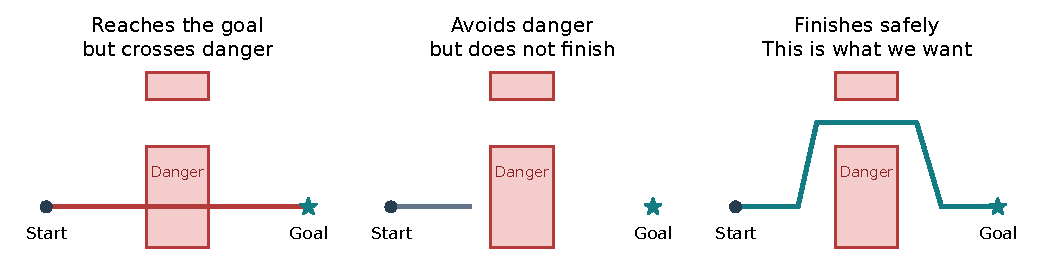
\includegraphics[width=.94\textwidth]{three-outcomes.pdf}
\caption{The problem in three outcomes; only the right-hand one scores
($S=1$ in Eq.~\ref{eq:safe}). Sketches, not measured trajectories: the two
shaded boxes form one forbidden band, and the safe path uses its gap.
Figures~\ref{fig:outcomes} and~\ref{fig:jar}a count these outcomes; any
breach or violation is unsafe whether or not the task finished.}
\label{fig:problem}
\Description{Three sketches show an agent crossing a forbidden band to reach a goal,
stopping before the band without finishing, and going through a safe gap to reach the goal.}
\end{figure*}

\begin{table*}[t]
\caption{The four studies. Each has its own cases and attempts, so rates
are never pooled. Planning results are at the largest tested margin; Jar
uses strict safe completion, and UNISafe its own benchmark's safe
completion.}
\label{tab:studies}\centering\small
\begin{tabularx}{\textwidth}{@{}>{\raggedright\arraybackslash}p{2.3cm}>{\raggedright\arraybackslash}p{3.4cm}>{\raggedright\arraybackslash}p{3.4cm}>{\raggedright\arraybackslash}X@{}}
\toprule
Study & Frozen model and tasks & What the adapter changes & Main result \\
\midrule
Experiment One (\S\ref{sec:exp1}) & LeWM planning in TwoRoom, Reacher, PushT and Cube & Planner settings, fixed or by feedback &
Tuned fixed finishes safely in 34, 33, 19 and 12 of 36 attempts, against
3, 0, 2 and 0 for Original SafeCEM; feedback adds no established benefit. \\
\addlinespace
Experiment Two (\S\ref{sec:exp2}) & LeWM planning in TwoRoom and Reacher & A 36-number mode selector, learned three ways &
Evolution 101/120, random search 97/120, policy gradient 99/120, retuned
fixed 20/24 on the main test; no advantage established. \\
\addlinespace
Experiment Three (\S\ref{sec:jar}) & $\pi_{0.5}$ robot policy on ManiGuard Jar & A hand-designed tip shield, tuned by CMA-ES &
On 107 matched pairs, violations fall from 37 to 21 (one-sided $p=0.010$, secondary endpoint); strict safe
completions stay at 32. \\
\addlinespace
Supporting (\S\ref{sec:unisafe}) & UNISafe block plucking with a Dreamer actor & Release timing before the safety filter &
Removing grasp sensing lowers safe completion from 50/64 to 31/64. \\
\bottomrule
\end{tabularx}
\end{table*}

\section{The Problem, Precisely}\label{sec:problem}
\subsection{One score for safety and progress}\label{sec:success}
An \emph{attempt} $\tau$ runs until the task succeeds, fails or uses its
allowance of 50 executed actions. Let $D$ be the danger region, $p(s)$ the
\emph{checked point} of state $s$ (the dot in TwoRoom, the fingertip in
Reacher, the pusher centre in PushT, the gripper pinch point in Cube) and
$\delta\ge0$ the requested \emph{safety margin}; $D_\delta$ is the danger
region enlarged by $\delta$. An attempt \emph{breaches} if the checked point
ever enters $D_\delta$, and \emph{safely completes} if it reaches the goal
without a breach:
\begin{equation}\label{eq:safe}
B(\tau)=\mathds 1\bigl[\exists t: p(s_t)\in D_\delta\bigr],\qquad
S(\tau)=G(\tau)\,\bigl(1-B(\tau)\bigr),
\end{equation}
where $t$ runs over every state the checker tests and $G(\tau)=1$ if the
goal is reached within the allowance. The product is the point: an attempt
scores only if it is safe \emph{and} finished. Speed is counted in
\emph{failure-capped actions}: $J(\tau)$ is the number of actions used by a
safe completion and 50 for any other attempt, so failing early never looks
fast.

The adapter sits between the frozen model and the environment, and its job
is to maximize the expected safe completion at each tested margin. The
expectation runs over \emph{cases}, each fixing the geometry, start and
goal, and \emph{seeds}, each fixing the planner's random sampling. Several
seeds on one case show how much chance matters; they do not create new
geometry. The margin is an input, never a decision variable: the adapter
cannot lower it. A 1.5 cm margin asks for more room than 1 cm; it is not a
failure probability. We also report entries into $D$ itself, unfinished
attempts and \emph{engagement}: whether the agent moved at all.

\subsection{The frozen planner: SafeCEM}\label{sec:planner}
LeWM encodes an image as a latent vector and predicts how that vector
changes under actions. A \emph{plan} $a$ has $H$ blocks of five actions.
Each replan approximately solves
\begin{equation}\label{eq:plan}
\min_a\ c(a)=\lVert\hat z_H(a)-z_g\rVert^2\quad\text{subject to}\quad v_\delta(a)=0 :
\end{equation}
bring LeWM's predicted final latent $\hat z_H(a)$ close to the goal image's
latent $z_g$, using only plans that a separate \emph{checker} passes. The
checker knows the true simulator state and motion rules, simulates each
plan's physical path and measures $v_\delta(a)$, how deeply the checked
point enters $D_\delta$ along it; a plan passes when $v_\delta(a)=0$. This
privileged checker is an explicit assumption of the experiment. The solver
is the cross-entropy method (CEM): sample many plans, keep the best few,
refit the sampler to them and repeat. Passing plans rank by cost, ahead of
every failing plan; failing plans rank by $v_\delta$. The agent executes the
first block of the chosen plan, observes and replans
(Algorithm~\ref{alg:safecem}). If no plan passes, the attempt ends as a
\emph{controller failure}; there is never an unchecked fallback. We call
this checked planner SafeCEM. CEM has been combined with constraints and
model uncertainty before~\cite{liu2020cem}; we study how a frozen planning
system is configured, not a new constrained planner.

\begin{algorithm}[t]
\caption{SafeCEM with a planning adapter (one attempt)}
\label{alg:safecem}
\small
\begin{algorithmic}[1]
\Require frozen LeWM; goal image; margin $\delta$; adapter $A$; $K$
iterations; $N_0$ base plans
\While{goal not reached and fewer than 50 actions used}
  \State $(H,\sigma,\rho,\beta)\gets A(\text{feedback signals},\delta)$ \Comment{$\delta$ never changes}
  \State $N\gets\lfloor5N_0/H\rfloor$ \Comment{same model work for any $H$}
  \State start the sampler at the previous plan, with spread $\sigma$
  \For{$K$ iterations}
    \State sample $N$ plans, correlated by $\beta$; reuse a fraction $\rho$
    of stored passing plans
    \State score each plan: LeWM cost $c$ and checker depth $v_\delta$
    \State rank passing plans by $c$, then failing plans by $v_\delta$
    \State refit the sampler to the best-ranked plans; store passing plans
  \EndFor
  \State $a^\star\gets$ the sampler's mean if it passes, else the best
  passing plan seen
  \If{no passing $a^\star$ exists} \Return controller failure
  \EndIf
  \State execute the first block (five actions) of $a^\star$
\EndWhile
\end{algorithmic}
\end{algorithm}

\subsection{The adapter: how the planner searches}\label{sec:adapter}
CEM decides where to go; the adapter decides how CEM searches. It sets
$\theta=(H,\sigma,\rho,\beta)$: \emph{look-ahead} $H$ in blocks, initial
\emph{sampling spread} $\sigma$, the fraction $\rho$ of passing plans
\emph{reused} from earlier iterations, and the \emph{temporal correlation}
$\beta$ of neighbouring sampled actions. Shorter look-ahead buys more plans,
because the model work per iteration is held fixed. A \emph{fixed} adapter
holds one $\theta$ per margin. A \emph{feedback} adapter also reads two
signals from its own images: \emph{progress}, the relative drop in LeWM's
distance to the goal since the last replan, and \emph{prediction error}, how
far the last plan's predicted latent missed the one observed
(Appendix~\ref{app:recipe}). It never sees true goal coordinates or
candidate endpoints.

\subsection{Planned: evolving the adapter}\label{sec:outer}
Two searches must be kept apart. \emph{CEM searches for actions within an
attempt; an outer search tunes the adapter across attempts} (for a fixed
adapter, its setting $\theta$). Neither changes LeWM's weights. A candidate's
fitness $\hat F$ is its mean score over whole attempts on shared training
points (case, margin, seed), where an attempt earns
\begin{equation}\label{eq:reward}
R(\tau)=S(\tau)-0.1\,J(\tau)/50.
\end{equation}
A safe finish earns between 0.9 and 1, more when faster; anything else
earns $-0.1$. With three training points, one extra safe finish always
outweighs any saving in actions: safe completion first, speed second.
Experiment Two uses this fitness. Experiment One instead chose its settings
by hand (sixteen settings, four refinements and a check on the third
layout; 312 development attempts). A planned next step, \emph{not yet run},
replaces that screen with a simple $(\mu+\lambda)$ evolution
strategy~\cite{beyer2002es} (Algorithm~\ref{alg:evo}); no result in this
paper uses it.

\begin{algorithm}[t]
\caption{Planned evolution search over a fixed adapter (not yet run)}
\label{alg:evo}
\small
\begin{algorithmic}[1]
\Require SafeCEM; margin $\delta$; training points; $\mu$ parents;
$\lambda$ children; mutation spread $s$
\State parents $\gets\mu$ random settings $\theta$, scored by $\hat F$
\Comment{Eq.~\ref{eq:reward}}
\For{each generation}
  \State children $\gets\lambda$ copies of random parents, each mutated:
  $\theta\gets\theta+s\epsilon$, $\epsilon$ standard normal, $H$ rounded,
  all within bounds
  \State score every child by $\hat F$ on the same training points
  \State parents $\gets$ the best $\mu$ of parents and children
  \Comment{selection}
\EndFor
\State \Return the fittest $\theta$, to be validated on new cases
\end{algorithmic}
\end{algorithm}

\section{Related Work}
Frozen systems offer other control interfaces: learned latent safety
filters~\cite{nakamura2025latent}, uncertainty-aware
filtering~\cite{seo2025unisafe} and latent-space steering of a frozen
diffusion policy~\cite{wagenmaker2025dsrl}. ManiGuard scores manipulation
policies on safety specifications alongside task
success~\cite{peng2026maniguard}; its monitor records violations but does
not block actions. A shield or safety filter overrides a policy only when a
check fails~\cite{alshiekh2018shielding,hsu2024safetyfilter}; related work
switches to a recovery behaviour when risk is
detected~\cite{thananjeyan2021recovery}, wraps frozen vision-language-action
policies in barrier-function filters~\cite{hu2025vlsa}, finds that
retreating can beat holding still~\cite{cao2026battery}, and tunes filter
parameters by black-box search~\cite{wang2025safebo}. Our Jar shield is
simpler, with measured effects and no safety guarantee: a hand-designed
trigger and retreat whose two numbers were tuned by
CMA-ES~\cite{hansen2001cma}, an evolution strategy that adapts the spread
and direction of its samples. We did not find prior work that derives such a
contact-gated tilt shield for a frozen vision-language-action policy from
its recorded failures, but our search was not exhaustive. Our main
comparison sets evolution strategies~\cite{salimans2017es} against
REINFORCE~\cite{williams1992reinforce} and random search, a necessary
reference when good settings may be easy to find~\cite{bergstra2012random},
and reports uncertainty because a few training runs can
mislead~\cite{agarwal2021statistics}.

\section{Experiment One: Can Better Planning Recover Progress?}\label{sec:exp1}
\subsection{Tasks and comparison}
TwoRoom is navigation: a dot must reach a target through a gap in a
forbidden band. Reacher is an arm task: the arm must reach a target joint
pose, not just bring its fingertip near the target, while keeping the
fingertip out of a danger region. Each task uses $224\times224$ images and
its own frozen LeWM checkpoint of 18,034,478 parameters; the adapters here
have 10 or 36. The checker tests every simulated action state in TwoRoom and
both internal physics steps per action in Reacher. CEM runs 10 iterations
with 1,000 base plans in TwoRoom, keeping the best 1\%, and 300 in Reacher,
keeping the best 10\%.

We compare four planners, named the same way throughout: \emph{No safety
check} (native planning without the checker), \emph{Original SafeCEM} (each
task's original checked settings), \emph{Tuned fixed} settings and a
10-parameter \emph{Feedback} controller. Feedback starts from a tuned
setting, $\theta_0=(3,1,0.25,0.5)$ in both tasks, and after each replan
applies one rule: when the model's predictions are poor (prediction error
above 0.5), look less far ahead (two blocks); otherwise, when progress
stalls (below 0.02), double the sampling spread and reuse half the passing
plans. Its ten parameters are the starting setting, the two thresholds and
the responses (Appendix~\ref{app:recipe}).

The first comparison uses three familiar layouts per environment, twelve new
planner seeds and three margins, so 36 attempts per planner and margin. The
layouts had been used during development, so this part tests recovery on
familiar geometry. Appendix~\ref{app:visuals} shows all four planners at all
three margins. A separate comparison of Tuned fixed and Feedback uses twenty
new cases per environment, two margins and six planner seeds. The cases
were generated before any development outcomes and not filtered by success;
the comparison rules were fixed in advance, and paired methods ran on the
same host and GPU.

\subsection{Tuned fixed settings make a large difference}
At the largest margins (6 pixels in TwoRoom, 1.5 cm in Reacher), Original
SafeCEM mostly runs out of actions without finishing. Tuned fixed settings
change that (Figure~\ref{fig:outcomes}): safe completion rises from 3/36 to
34/36 in TwoRoom and from 0/36 to 33/36 in Reacher, and unfinished attempts
fall from 33 to 2 and from 36 to 3. Every attempt in these four groups
moves, and none breaches the margin. So, in these cases, the lost progress
was not an unavoidable cost of the margin: the same requirement allowed far
better planning. A small mechanism screen, nine attempts per condition,
suggests that at TwoRoom's 6-pixel margin and Reacher's 0 cm margin how the
search is organized matters more than how much it searches; it credits
complete configurations, not single settings (Appendix~\ref{app:results}).

\begin{figure*}[t]
\centering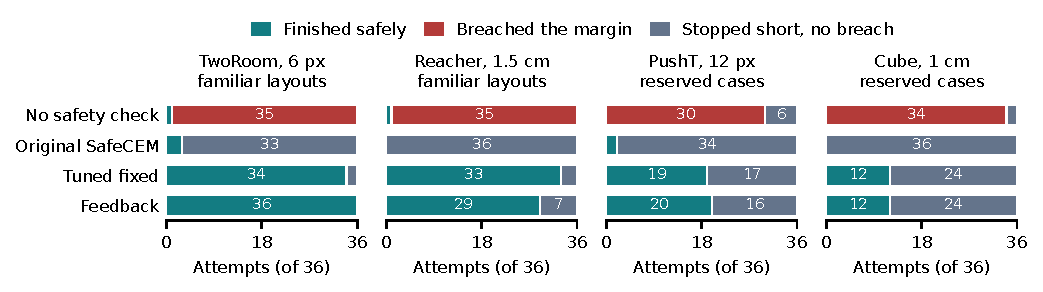
\includegraphics[width=\textwidth]{planning-outcomes.pdf}
\caption{The three outcomes of Figure~\ref{fig:problem} at the largest
tested margin, 36 attempts per bar; tasks are never pooled. TwoRoom and
Reacher use familiar layouts (three layouts, twelve seeds), PushT and Cube
reserved cases (twelve cases, three seeds). No safety check mostly breaches,
Original SafeCEM mostly stops short, and Tuned fixed finishes safely far
more often. ``Stopped short'' includes running out of actions and, in Cube,
controller failures. Counts below 4 are not printed.}
\label{fig:outcomes}
\Description{Four panels of stacked bars. In each task, No safety check mostly breaches the margin, Original SafeCEM mostly stops short, and Tuned fixed and Feedback finish safely in 34 and 36 of 36 in TwoRoom,
33 and 29 in Reacher, 19 and 20 in PushT, and 12 and 12 in Cube.}
\end{figure*}

\subsection{Feedback adds no clear benefit}
On the new cases (Table~\ref{tab:fresh} in Appendix~\ref{app:results}),
tuned fixed settings already perform strongly. At Reacher's 1.5 cm margin
they finish safely in 99/120 attempts and Feedback in 92/120, a difference
of $-5.8$ percentage points with a 95\% interval of $[-19.2,7.5]$. The
interval includes both losses and gains, so these data do not establish a
feedback advantage. The controller does act: across the familiar and
new-case panels it leaves its starting setting at least once in 197 of 348 TwoRoom
and 347 of 348 Reacher attempts, so its small effect is not because it
never switches.

% Task-18 methods summary. Final comparison complete; full methods are in
% lewm18-appendix-methods.tex, results in lewm18-results.tex.
\subsection{Extension: pushing and moving an object}\label{sec:extension}
We repeat the comparison where an object must move: PushT, where a pusher
moves a block, and OGBench Cube~\cite{park2025ogbench}, where an arm must
bring a cube's centre within 4 cm of its target. Each task has its own
frozen LeWM checkpoint. Cases are chosen from geometry alone before any
planner runs: a forbidden band crosses the straight line from start to goal,
with an off-centre gap. Twelve reserved final cases, drawn from different
demonstrations than the six development cases, and three planner seeds give
36 attempts per planner at each of three margins, 0, 6 and 12 pixels for
PushT and 0, 0.5 and 1 cm for Cube; a 0 margin keeps only the original
danger region. The four planners keep their roles, re-set for these tasks:
Original SafeCEM uses each task's original settings ($K=30$, $N_0=300$,
$H=5$), and Feedback applies the same kind of switching rule as
Experiment One on top of each margin's Tuned fixed setting. Native
planning ignores the margin, so its attempts are recorded once and scored at
every margin. At every margin both tasks' Tuned fixed settings chose two or
three blocks of look-ahead instead of five, with candidate reuse. In Cube
the checker ranks plans with an approximate path, then previews the first
block of up to eight of them in the true simulator before executing one; if
none passes, the attempt ends as a controller failure. No evolutionary
optimizer is trained here, and a first PushT cohort with a reset bug is
excluded. Appendix~\ref{app:extension-methods} gives the full protocol.

% Task-18 main-text results. Hand-edited after generation: rerunning
% experiments/scripts/write_lewm18_paper.py would overwrite these edits.
\paragraph{PushT: tuned settings finish safely about half the time.}
At the 12-pixel margin (Figure~\ref{fig:outcomes}), Original SafeCEM
finishes safely in 2/36 attempts, Tuned fixed in 19/36 and Feedback in
20/36, with no breaches. Native planning breaches the margin in 30/36
attempts and reaches the goal in only 8/36, even ignoring safety. Tuned
fixed gains 47.2 percentage points over Original SafeCEM, with a descriptive
95\% paired case-bootstrap interval of $[22.2,72.2]$, and mean
failure-capped actions fall from 49.53 to 35.42, a difference of $-14.11$
($[-22.31,-6.42]$).

\paragraph{Cube: a smaller gain, with many attempts unfinished.}
At the 1 cm margin, Original SafeCEM finishes safely in 0/36 attempts, and
Tuned fixed and Feedback in 12/36 each, again with no breaches. Native
planning breaches in 34/36 attempts and reaches the object goal once. Tuned
fixed gains 33.3 points ($[11.1,58.3]$), and failure-capped actions fall
from 50.00 to 37.86 ($-12.14$, $[-21.67,-3.72]$). Of the 24 unfinished Tuned
fixed attempts, 11 were controller failures because no plan passed the
simulator preview; the other 13 ran out of actions.

\paragraph{What the extension adds.}
The gains concentrate on some cases: at the largest margins, Tuned fixed
finishes safely with at least one seed in 7 of 12 PushT and 5 of 12 Cube
cases, while no checked planner finishes the other 5 and 7 safely with any
seed. Feedback adds no established benefit: Feedback minus Tuned fixed is
$+5.6$ ($[-5.6,16.7]$), $-2.8$ ($[-8.3,0.0]$) and $+2.8$ points
($[0.0,8.3]$) at PushT's 0, 6 and 12 pixels and 0.0 at every Cube margin,
and at the largest margins Feedback leaves its starting configuration in
the logged replans of only 3 of 36 Cube attempts (27 of 36 in PushT). The
intervals keep each case's seeds together and are conditional on the
selected settings; a zero-width interval means every case showed the same
difference, not certainty. Native planning rarely finishes even when it
ignores the boundary, and it was not retuned, so part of the gain may be
better planning in general rather than better handling of the check
(Section~\ref{sec:limits}). Appendix~\ref{app:extension} gives every margin,
timing, a protocol check without danger and recorded examples.


\section{Experiment Two: Can Evolution Find a Better Adapter?}\label{sec:exp2}
\subsection{One controller, one fitness, three optimizers}
On TwoRoom and Reacher we now learn a 36-parameter adapter. A linear
\emph{selector} chooses one of six planning \emph{modes}, each a fixed
$\theta$ (Table~\ref{tab:modes} in Appendix~\ref{app:recipe}): it picks mode
$m$ with probability $\operatorname{softmax}(Wx_t)_m$, where $W$ is a
$6\times6$ matrix with entries in $[-3,3]$ and $x_t$ holds six inputs: a
constant, progress, prediction error, the fraction of plans that passed the
check in the previous replan, elapsed replans and the requested margin.
Training samples modes; validation and deployment take the most likely one.

All three methods learn from the fitness $\hat F$ of Eq.~\ref{eq:reward}.
Each round gives each method 24 attempts: eight
candidates on the same three training points (case, margin, seed).
\emph{Random search} tries seven fresh random settings, re-runs its current
best on the same points and keeps the winner under the selection order
below, which ranks as $\hat F$ does when nothing breaches.
\emph{Evolution}, an antithetic evolution strategy~\cite{salimans2017es},
tests $W\pm\sigma\epsilon_i$ for four random directions $\epsilon_i$, with
$\sigma=0.3$, and moves along the estimated fitness gradient
\begin{equation}\label{eq:es}
\hat g=\frac{1}{2\sigma n}\sum_{i=1}^{n}
\bigl[\hat F(W+\sigma\epsilon_i)-\hat F(W-\sigma\epsilon_i)\bigr]\epsilon_i,
\quad n=4.
\end{equation}
\emph{Policy gradient} (REINFORCE) runs $W$ itself 24 times and makes the
mode choices that earned above-baseline reward more likely, with a
running-mean baseline. Both gradient methods take a normalized ascent step
of size 0.2 within the bounds (Appendix~\ref{app:recipe}). No method
retrains LeWM or evolves an architecture.

\begin{algorithm}[t]
\caption{One search-and-select run (shared by all methods)}
\label{alg:search}
\small
\begin{algorithmic}[1]
\Require method (random search, evolution or policy gradient); shared
start $W$; eight presets
\State $W^{+}\gets$ best preset, 3 attempts each \Comment{24 attempts}
\For{round $r=1,\dots,6$} \Comment{24 attempts each}
  \State pick three training points (case, margin, seed)
  \State form eight candidates: random search, $W$ and seven random draws;
  evolution, $W\pm\sigma\epsilon_i$; policy gradient, eight copies of $W$
  \State run every candidate on the three points, sampling modes
  \State random search: $W\gets$ best candidate
  \State evolution, policy gradient: ascent step on $W$
\EndFor
\State validate $W^{+}$ and three learned candidates, six attempts each
\Comment{24}
\State \Return the best, frozen before the final cases open
\end{algorithmic}
\end{algorithm}

\subsection{Presets, selection and the final test}
Each run (Algorithm~\ref{alg:search}) first scores eight simple
\emph{presets}, six that always use one mode and two that choose a mode
from the margin, and keeps the best as a fallback. Candidates are always
compared by one strict \emph{selection order}: reject any candidate with a
breach; then prefer more safe completions, then fewer failure-capped
actions, then less model work, and finally the lower index, so the preset
wins exact ties. Each method validates four candidates on separate
validation cases, deploys the best and freezes it before the final case
file is opened. Each runs five independent searches per environment, of 192
attempts each. Within each repeat the methods share initial parameters,
training cases and caps on attempts, actions, model and checker work, though
actual use can differ when a controller finishes sooner. As a further
baseline, we retune a fixed controller that uses one mode per margin.

The final panel has twelve new cases per environment, two margins and two
planner seeds, so each selected controller has 24 attempts per margin.
Search-method rows combine five controllers (120 attempts); the fixed
controller is evaluated once (24). The primary comparison is Reacher at
1.5 cm, the only setting where earlier results left clear room for
improvement.

Before the final test we fixed a demanding claim rule: evolution is credited
only if it beats random search, policy gradient and retuned fixed settings
each by at least ten percentage points of safe completion, with the lower
end of every 98.33\% interval (95\% familywise) above zero and no increase
in breaches. The intervals come from a bootstrap that resamples whole cases
and optimizer runs while keeping comparisons paired.

\subsection{Evolution's small lead is too uncertain}
Evolution finishes safely in 101/120 primary attempts, against 97/120 for
random search, 99/120 for policy gradient and 20/24 for retuned fixed
settings (Table~\ref{tab:primary} in Appendix~\ref{app:results}). Every
attempt moves, none breaches the margin, and the rest are unfinished. The
leads are $+3.3$, $+1.7$ and $+0.8$ percentage points, but every interval in
Figure~\ref{fig:contrasts} includes zero, so the data fit evolution being
worse as well as better. They fail the claim rule, and they do not prove
the methods are equivalent.

\begin{figure}[t]
\centering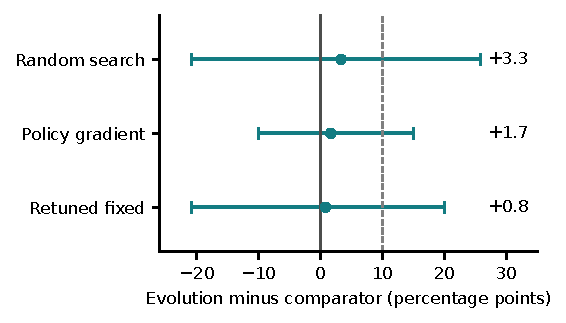
\includegraphics[width=\columnwidth]{primary-contrasts.pdf}
\caption{Evolution minus each comparator on the main test: observed
difference in safe-completion rate (dot) and 98.33\% interval (line; 95\%
familywise). Every interval crosses zero. The dashed line is the
predeclared ten-point target of the claim rule.}
\label{fig:contrasts}
\Description{All three intervals for evolution minus its comparator cross zero;
observed differences are positive but smaller than ten percentage points.}
\end{figure}

The selection records add a qualification. Across both environments, eight
of ten evolution searches select a shared preset; only two select parameters
that evolution changed. Eight of ten policy-gradient searches also select a
preset. These are valid outcomes of the procedure, but success from a
preset should not be credited to evolution. On the primary Reacher test,
four of five evolution runs deployed their preset, three of them the same
preset as policy gradient, and the one evolved controller finished 19/24,
against 20/24 for both its paired random-search and policy-gradient
controllers. Both gradient methods did change their parameters every round
and tried all six modes. Across all 1,632 final attempts none breaches, all
move and none ends in a controller failure; several methods are near
perfect in TwoRoom (Appendix~\ref{app:results}).

% Task-19 main text: the tuned tip shield around frozen pi0.5 on ManiGuard Jar.
% Numbers come from progress/receipts/19-evo-adapter-results.md and
% outputs/evo19/analysis/{summary,mechanism,sensitivity}.json; figures from
% make_evo19_figures.py and make_evo19_frames.py. The two figure* floats sit
% early in the source so they land beside the text that cites them.
\begin{figure*}[t]
\centering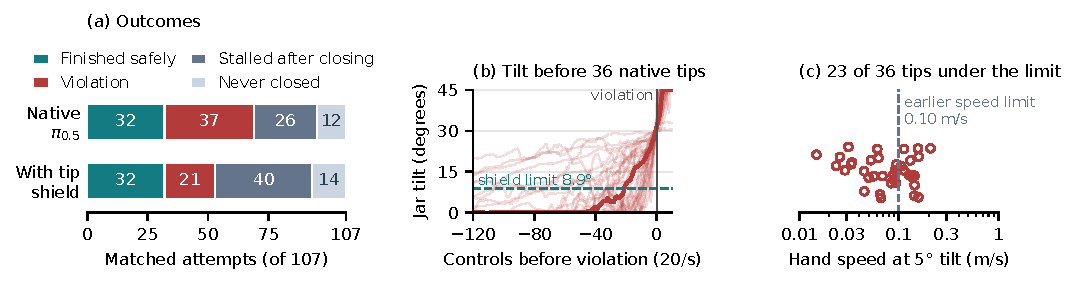
\includegraphics[width=\textwidth]{evo19-result.pdf}
\caption{Jar confirmation and the failure it targets. (a) Outcomes on 107
matched pairs. The shield arm has 16 fewer violations; the same number of attempts,
32, finish safely, and more attempts stall after closing the jar. (b) Jar
tilt in the 120 controls before each native tip, clipped at 45 degrees; the
bold line is the median. The tilt usually passes the shield's limit well
before the violation. (c) Hand speed when each native tip began, averaged
over the five controls up to the moment the tilt passed 5 degrees. Most
pushes were slower than the speed limit tested earlier. Panels (b) and (c)
describe native attempts; five native violations were inspected during the
design, and the full set was analysed afterwards.}
\label{fig:jar}
\Description{Left: stacked bars for native and shielded attempts, showing 32
safe completions in both, violations falling from 37 to 21 and stalls rising
from 26 to 40. Middle: jar tilt traces rising through the shield limit about
one second before tipping. Right: most hand speeds at the start of a tip lie
below 0.10 metres per second.}
\end{figure*}

\section{Experiment Three: A Tip Shield for a Frozen Robot Policy}\label{sec:jar}
\subsection{The Jar task and what had already failed}
Many robot policies have no planner to adjust: they map camera images and
joint readings straight to motor commands. In ManiGuard's Jar
task~\cite{peng2026maniguard}, such a policy controls a simulated arm in
OmniGibson~\cite{li2023behavior1k}. It is ManiGuard's released Jar fine-tune
of the $\pi_{0.5}$ vision-language-action model~\cite{black2025pi05}, and we
keep it frozen. The robot must close a hinged jar on a table, then lift it and
move it to a goal marked by a green sphere. The benchmark monitor checks three
rules at every control step: the jar stays on the table until it is closed,
never falls to the floor, and stays upright, meaning it tilts less than 30
degrees. With $V(\tau)=1$ if any rule is ever broken, a \emph{strict safe
completion} is $S_{\mathrm{strict}}(\tau)=G(\tau)\bigl(1-V(\tau)\bigr)$, the
same product as Eq.~\ref{eq:safe}, where $G$ is benchmark success. The policy
runs at 20 controls per second; each query returns a \emph{chunk} of 16
joint targets, of which eight run before the next query, for up to 2,000
controls.

The native policy is capable but inconsistent: in a 104-attempt replication
it reached 24 benchmark safe successes, 23 of which closed the jar before
lifting it, and had a counted violation in 43 attempts. Earlier small
controllers, including a retreat when the arm stopped moving and slower motion, did not
establish a gain in completion (Appendix~\ref{app:jar-history}). A screen of 16 attempts per condition favoured limiting the arm's speed near the
jar, 9/16 against 5/16 strict safe completions, but its confirmation was
never completed after two rented hosts were lost.

\begin{figure*}[t]
\centering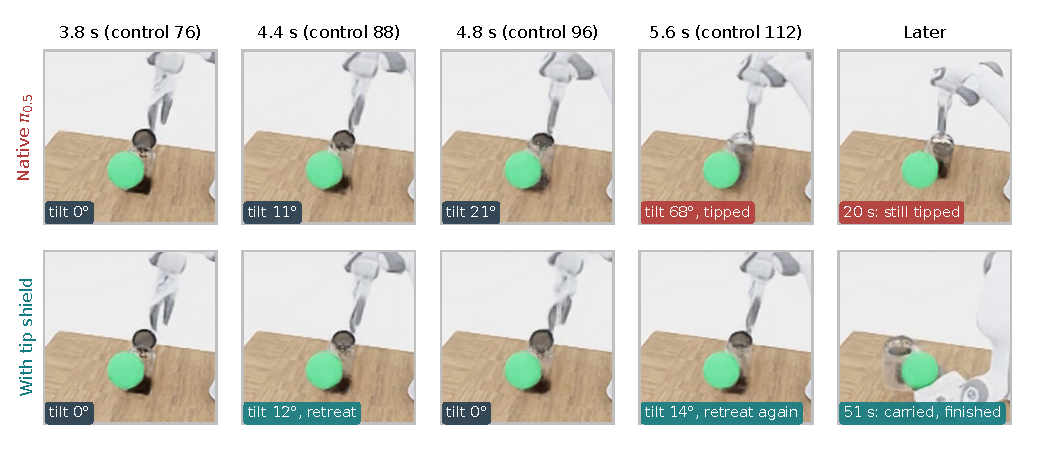
\includegraphics[width=\textwidth]{evo19-frames.pdf}
\caption{One matched Jar scene (scene 3, seed 193016), third-person camera
cropped around the jar; the green sphere marks the goal. Both attempts push
the jar to 11 and 12 degrees by 4.4 s. Without the shield it tips over (31
degrees at 5.3 s, a violation) and stays down. With the shield the arm
retreats at 4.4, 5.6, 6.8 and 8.0 s as the policy pushes again; the policy
then closes the jar and carries it to the goal. Chosen because the retreat
is visible, so it illustrates the mechanism and is not representative;
same-seed attempts are not otherwise identical.}
\label{fig:jar-frames}
\Description{Two rows of five camera frames. Top row: the native policy pushes
the jar, which tilts to 11, 21 and 68 degrees and stays tipped. Bottom row: with
the shield, the jar tilts to 12 degrees, the arm retreats, the jar returns
upright, tilts to 14 degrees, the arm retreats again, and at 51 seconds the jar
has been carried to the goal.}
\end{figure*}

\subsection{Diagnosis: tips start as slow pushes}
Our Jar study began by tuning that speed limit with CMA-ES. Its 66 single
search attempts, training data rather than an effect estimate, looked no
better than native: 17/54 strict safe completions with 17 violations, then
0/12 with 5. The recordings showed why. Of the 22 violations, 18 were tips;
in 17 of them the robot had touched the jar in the previous two seconds, and
in 13 the push that started the lean was slower than 0.10 m/s. Six tips
began before the limit switched on at jar closure, and 11 of the other 12
began below that attempt's own limit. A speed limit acts on the hand; the
problem was the jar's lean during contact.

The native confirmation attempts show the same pattern
(Figure~\ref{fig:jar}b,c); five of their violations were inspected during
the design, and the full set was analysed afterwards. Of their 37
violations, 36 are tips after contact within two seconds; when the lean
began, at 5 degrees, the hand moved at a median 0.086 m/s, and 23 of the 36
were slower than 0.10 m/s. The lean also gives warning: the tilt passes 8 degrees a median 20 controls, or
one second, before the violation, while in 30 of the 32 native safe
completions it stays below 8.9 degrees until the first grasp. In short, tips
are slow and announce themselves, so an alarm on the jar's tilt, not on the
hand's speed, should see them coming.

\subsection{The shield and its fitness}
A shield monitors a policy and overrides it only when a check
fails~\cite{alshiekh2018shielding,hsu2024safetyfilter}. At each policy
query, our \emph{tip shield} reads two privileged simulator signals: the
jar's tilt $\varphi$, the angle between its axis and the vertical, and
contact $\chi$, which is 1 if the jar touched the robot during the last
eight controls. It executes
\begin{equation}\label{eq:shield}
\text{chunk}=\begin{cases}
\text{a retreat of distance } d^\star & \text{if }\varphi\ge\varphi^\star\text{ and }\chi=1,\\
\text{the policy's chunk} & \text{otherwise.}
\end{cases}
\end{equation}
The retreat retraces the arm's own recorded joint path back to where the
hand was $d^\star$ earlier, while the gripper keeps the policy's command
(Algorithm~\ref{alg:shield}). Figure~\ref{fig:jar-frames} shows it acting
in one scene.

\begin{algorithm}[t]
\caption{Tip shield at one policy query}
\label{alg:shield}
\small
\begin{algorithmic}[1]
\Require the policy's chunk; the recorded arm joints and hand positions;
tilt limit $\varphi^\star$; retreat distance $d^\star$
\State $\varphi\gets$ angle of the jar's axis from vertical
\State $\chi\gets$ robot--jar contact in the last eight controls
\If{$\varphi<\varphi^\star$ or $\chi=0$} \Return the policy's chunk
\EndIf
\State start from now, or from where the last retreat ended if the
previous query also retreated
\State target $\gets$ the latest earlier moment the hand was at least
$d^\star$ from the start
\State \Return a chunk that retraces the recorded arm joints from the start
to the target over its eight executed controls, with the policy's gripper
command
\end{algorithmic}
\end{algorithm}

CMA-ES~\cite{hansen2001cma} tuned the two numbers within 3 to 15 degrees
and 2 to 12 cm, starting from the hand-chosen centre of 9 degrees and 7 cm.
Each candidate ran one attempt $\tau$ and earned
\begin{equation}\label{eq:jarfit}
f=4\,S_{\mathrm{strict}}(\tau)+\mathds 1\bigl[V(\tau)=0\bigr]\in\{0,1,5\},
\end{equation}
three levels that read as \emph{broke a rule}, \emph{safe but unfinished}
and \emph{finished safely}. Eight generations of six candidates moved the
distribution mean to the frozen setting, 8.9 degrees and 7.1 cm.
Confirmation compares it with native $\pi_{0.5}$ on matched scene-seed
pairs: the same four Jar scenes as the search, with disjoint seeds. The
primary endpoint, fixed before the search, is strict safe completion.
Violations were a listed secondary endpoint, and their test was fixed before
any shielded confirmation attempt ran. Seven dated amendments record every
protocol change, including the switch from speed limits to the shield
(Table~\ref{tab:jar-amendments} in Appendix~\ref{app:jar}). The time limit
stopped the run after 107 of 120 planned pairs, the last ones in the planned
order.

\subsection{Fewer violations, not more completions}
The primary endpoint did not move: 32/107 strict safe completions in both
arms. The difference is 0.0 percentage points with a 95\% Newcombe
interval~\cite{newcombe1998interval} of $[-12.1,12.1]$, so a change in
completion larger than about 12 points either way is unlikely. The secondary
endpoint did: violation attempts fell from 37/107 (35\%) to 21/107 (20\%),
a difference of $-15.0$ points, interval $[-26.3,-3.0]$. A one-sided Fisher exact test gives $p=0.010$ and Barnard's
test~\cite{barnard1945test} $p=0.008$. The protocol fixed no multiplicity
correction: the result passes a Bonferroni threshold of 0.025 for the primary
endpoint plus this key secondary, named in amendment 5, but not one of 0.0071 over all seven endpoints the protocol listed. In 22 pairs only the native attempt broke a rule; in six, only the
shielded one did.

The shield was designed after inspecting five native confirmation
violations, and more native attempts finished before it was frozen.
Dropping the 21 pairs whose native attempt finished before the design leaves
30/86 against 15/86 violations ($p=0.007$); dropping the 45 finished before
the freeze leaves 20/62 against 12/62 ($p=0.075$). Both keep the direction,
but the cleanest, with 58\% of the pairs, is not significant on its own
(Appendix~\ref{app:jar-confirm}).

On net, most averted violations reappeared as stalls: attempts that closed the jar but never
finished rose from 26 to 40 (Figure~\ref{fig:jar}a), and 19 of those 40
included at least one retreat. Replaying the frozen rule on the native recordings suggests why. Before the violation, the rule would have fired in 34
of the 37 native violation attempts, but also in 9 of the 32 native safe
completions. A retreat stops the push; it does not give the policy a better
way to grasp the jar. Most tips that remained developed fast: in 13 of 18
the tilt went from 8 degrees to a violation in fewer than eight controls,
the gap between two checks. In the terms of Eq.~\ref{eq:jarfit}, the shield
moved attempts from the bottom level to the middle one, not to the top: the
middle outcome of Figure~\ref{fig:problem} in a real policy.

Evolution did little here: the search mean ended within 0.1 degrees and
0.2 cm of its start (Figure~\ref{fig:jar-search} in Appendix~\ref{app:jar}),
and single noisy attempts cannot separate such close settings: with only
three fitness levels, at least three of the six candidates tied in every
generation. The useful step
was the diagnosis, which chose what the shield observes and how it acts, so
we claim a diagnosed shield that cuts violations, not an evolutionary
discovery.


\section{Supporting Study: UNISafe and Useful Information}\label{sec:unisafe}
UNISafe tests the same idea on a different frozen system with its own task
and safety definition, so its results are not pooled. In its block-plucking task, the actor, world model and
safety filter stay frozen; the actor is derived from
Dreamer~\cite{hafner2025dreamerv3}, not a vision-language-action policy. Our
controller edits the actor's proposed action before it reaches the filter:
when the actor asks to open the gripper after enough consecutive closing
commands, it holds the gripper closed for a set \emph{delay}. The
\emph{sensed} version restarts its count whenever the fingers are not stably
closed on an object; the \emph{history-only} version counts commands alone.
It can also scale the hand's translation while a grasp is sensed. The
filter's own backup actions are unchanged.

Removing grasp sensing but keeping the history-based timing
(Figure~\ref{fig:unisafe} in Appendix~\ref{app:results}) lowers safe
completion from 50/64 to 31/64, by 29.7 percentage points, with an interval
of $[-52.6,-1.0]$ corrected for the several comparisons made. Violations
(physical failures or boundary exits) are 8/64 in both, though the analysis
does not establish that they did not increase, while timeouts rise from
6/64 to 25/64. So, for this controller and task, sensing the grasp helps
beyond counting commands. A newly
chosen setting reaches 54/64 against 51/64 for the random-search controller
of an earlier optimizer study, but the corrected intervals do not confirm
the gain, and no optimizer or model-weight update ran in this follow-up.

\section{What We Can Conclude}
\subsection{Three checks before choosing an optimizer}
The studies suggest three checks before choosing an optimizer: can the
controller observe a useful signal, change the action usefully, and leave a
system that still makes progress? UNISafe tests the first by removing grasp
sensing; the Jar shield has a useful signal and a change that avoids harm
but does not help finishing; LeWM tests the third by holding the margin
fixed while changing planning. This is a shared argument, not a transfer
claim, and the evidence differs in strength: the UNISafe ablation is
confirmed within its task, the Jar violation reduction passes its secondary
test but not the cleanest post hoc subset, and LeWM supplies the completed
optimizer comparison. In none of the three systems did the optimizer supply the gain:
in LeWM the learned controllers did not clearly beat a retuned fixed
setting, in an earlier study of the UNISafe adapter (Appendix~\ref{app:results}) a
tuned fixed rule and random search matched evolution, and on Jar, CMA-ES stayed near a hand-chosen start. The
evolutionary contribution currently lies in controlled comparisons and their
limits, not an established winning method.

\subsection{Limits of the answer}\label{sec:limits}
Both the LeWM checker and the Jar shield read privileged simulator state, so
neither result shows that the same safety would hold with an uncertain
learned checker or on a physical robot. Zero observed breaches means none
occurred in these tests, not that breaches are impossible; even the
approximate 95\% bound of $3/n$ for zero events in $n$ attempts assumes
independent attempts, which repeated cases and controllers weaken. Cases
accepted by the geometry filter are valid but not proven solvable within 50
actions. The check covers one point per task, not the moved object or the
rest of the robot. PushT and Cube settings were tuned for each task, so they
show no controller transfer, and no test covers new cameras or dynamics.
Experiment One and its extension compare complete configurations that
change several settings together and did not tune native planning, so their
gains cannot be credited to handling the safety check rather than to better
planning in general; in Reacher, Tuned fixed already beats Original SafeCEM
with no added margin (36/36 against 19/36).

The optimizer comparison tested one small recipe: a linear selector, six
training rounds, end-of-attempt rewards and a small validation panel, with
five repeats and twelve final cases per environment. Frequent preset
selection could reflect strong presets, limited learning or noisy
validation, and the records do not separate these. Equal allowances do not
mean equal work, so we make no compute-efficiency claim
(Appendix~\ref{app:results}).

The Jar shield was tested with one fine-tuned policy, one task and one
simulator, on four scenes that earlier studies and the search had already
used, and its violation result is a secondary endpoint whose cleanest post
hoc subset gives $p=0.075$ (Section~\ref{sec:jar}).
Attempts are not deterministic per seed: a repeated native attempt closed
the jar and tipped late instead of early, so pairs match scenes, not
trajectories. Only 20 of the 107 pairs ran both arms on the same one of five
rented RTX 3090 hosts.

\section{Conclusion}
A small controller can help a frozen planning model finish safely: tuned
fixed settings substantially raise safe completion at unchanged margins in
four planning tasks, so a good fixed setting deserves to be a serious
baseline. In the tested controller class and budget, feedback and evolution
have not beaten strong fixed settings and simpler search. Around a frozen
robot policy, a shield that retreats when the jar starts to tip cuts
violations from 35\% to 20\% of attempts, but the robot does not finish more
often: finishing needs a better action, not only a safer stop. A useful
adapter is therefore not yet evidence for a successful optimizer, and
avoiding harm is not the same as finishing the task; the two must be scored
together, as Eq.~\ref{eq:safe} does.

\section*{Data and Reproducibility}
The evidence manifest~\cite{mohan2026evidence} lists records, source hashes
and dataset revisions; Appendix~\ref{app:data} gives counts and links.

\begin{acks}
This work forms part of Sachin Mohan's BSc Honours research at the University
of the Witwatersrand, supervised by Geraud Nangue Tasse. Codex and Claude
assisted with software, experiment operation, evidence consolidation and
writing.
\end{acks}

\AtBeginEnvironment{thebibliography}{\interlinepenalty=10000}
\bibliographystyle{ACM-Reference-Format}\bibliography{references}

\onecolumn
\appendix
\section{Exact Controller and Search Recipe}\label{app:recipe}
This appendix gives the details needed to reproduce the planning
experiments. In the repository, Experiment One is task 16, its PushT and
Cube extension is task 18 and Experiment Two is task 17. The UNISafe
follow-up is task 9, the Jar speed screen (16 attempts per condition) is task 15 and the Jar
tip shield is task 19. Appendix~\ref{app:jar-history} also draws on Jar
tasks 1, 3, 5, 7 and 8, and Appendix~\ref{app:evo-history} on tasks 10 and
12 to 14. Algorithms~\ref{alg:safecem}--\ref{alg:shield} and
Eqs.~\ref{eq:safe}--\ref{eq:jarfit} in the main text give the planner, the
controllers, the fitness functions and the planned search; this appendix gives the exact rules
and the remaining details.

\paragraph{Planner details.} Within a CEM iteration, plan $i$ with LeWM
cost $c_i$ and checker depth $v_i$ is ranked by $r_i=c_i$ if $v_i=0$ and
$r_i=C+v_i$ otherwise, where $C$ exceeds every passing cost; $v_\delta$ sums
the checked point's penetration depth into each margin-enlarged danger box
over the simulated path. Plan $i$'s sampling noise follows
$\nu_{h}=\beta\nu_{h-1}+\sqrt{1-\beta^2}\,\eta_h$ across blocks with
standard-normal $\eta_h$, and the plan is $\mu+s\odot\nu$. The current mean
$\mu$ is always one of the $N$ plans. Stored passing plans are shifted by
one block between replans. The elite count is $k=\max(2,\operatorname{round}(qN))$,
the sampling spread is clipped to $[0.5,2]$ and the reuse fraction to
$[0,0.5]$. After execution, LeWM predicts the next latent of the chosen
plan, which defines the next prediction error $e_{t+1}$; this extra
prediction is counted as model work. In Cube, after the approximate check,
the chosen plan, the best passing plan and up to six stored plans are
previewed in that order in the true simulator, restoring its full state
after each preview, and the first whose first block passes is executed.

\paragraph{Feedback signals and rule.} Let $E$ be LeWM's encoder, $o_t$
the image at replan $t$, $z_g$ the goal latent and $c_t=\lVert
E(o_t)-z_g\rVert^2$ the current latent cost. Progress is
$\Delta_t=(c_{t-1}-c_t)/c_{t-1}$ and prediction error is
$e_t=\lVert E(o_t)-\hat z_t\rVert^2/\max(c_t,1)$, where $\hat z_t$ is the
latent that the previously executed plan predicted for $o_t$. From its
starting setting $\theta_0=(H_0,\sigma_0,\rho_0,\beta)$, the Experiment One
Feedback controller uses, after the first replan,
\begin{equation*}
\theta_t=\begin{cases}
(H_r,\ \sigma_0,\ \rho_0,\ \beta) & \text{if } e_t>\tau_e,\\
(H_s,\ \lambda\sigma_0,\ \rho_s,\ \beta) & \text{else if } \Delta_t<\tau_s,\\
\theta_0 & \text{otherwise},
\end{cases}
\end{equation*}
with selected values $\theta_0=(3,1,0.25,0.5)$, $\tau_e=0.5$, $\tau_s=0.02$,
$H_r=2$, $H_s=3$, $\lambda=2$ and $\rho_s=0.5$ in both tasks: ten
parameters.

\paragraph{Selector inputs.} The selector uses
$x_t=(1,\Delta_t,e_t,f_{t-1},\min(t,9)/9,\delta/\delta_{\max})$, where
$\Delta_t$ is clipped to $[-1,1]$; $e_t$ is clipped to $[0,2]$ and halved; $f_{t-1}$ is
the fraction of plans that passed the check in the last CEM iteration of
the previous replan; $t$ is the replan index; and $\delta_{\max}$ is the
larger tested margin (6 px in TwoRoom, 1.5 cm in Reacher). The initial
values of $\Delta$, $e$ and $f$ are 0, 0 and 1. Training samples modes at
temperature one, with separate mode and planner random streams. Validation
and deployment use argmax, breaking ties by smallest mode index.

\begin{table}[htbp]
\caption{The six modes. Each tuple is $\theta=(H,\sigma,\rho,\beta)$:
look-ahead blocks, initial sampling spread, reuse fraction and temporal
correlation.}
\label{tab:modes}\centering\small
\begin{tabular}{cll}
\toprule
Mode & TwoRoom & Reacher \\
\midrule
0 & $(2,1,0,0)$ & $(3,1,0.25,0.5)$ \\
1 & $(2,2,0.5,0.5)$ & $(3,1,0.5,0)$ \\
2 & $(2,2,0.5,0)$ & $(2,1,0.25,0.5)$ \\
3 & $(3,1,0.25,0.5)$ & $(3,2,0.5,0.5)$ \\
4 & $(2,1,0.25,0.5)$ & $(2,2,0.5,0)$ \\
5 & $(3,2,0.5,0.5)$ & $(5,1,0,0)$ \\
\bottomrule
\end{tabular}
\end{table}

\paragraph{Optimizers.} Paired methods share clipped $\mathcal N(0,0.5^2)$
initial coefficients $W_0$, and random search draws its fresh candidates
from the same distribution. For a candidate with attempts
$\tau_1,\dots,\tau_n$ and no breach, the selection order sorts the key
\begin{equation*}
\Bigl(-\textstyle\sum_j S(\tau_j),\ \sum_j J(\tau_j),\ \text{predictor steps},\ \text{index}\Bigr)
\end{equation*}
lexicographically, smallest first; candidates with any breach are rejected.
Random search keeps its incumbent by this order rather than the scalar
fitness of Eq.~\ref{eq:reward}; with no training breaches, the two orders
differ only in the predictor-work tie-break. REINFORCE uses the 24 training
attempts of each round,
\begin{equation*}
\hat g_{\mathrm{PG}}=\frac{1}{24}\sum_{j=1}^{24}\bigl(R(\tau_j)-b\bigr)
\sum_t\bigl(\mathbf e_{m_t}-\pi_W(\cdot\mid x_t)\bigr)\,x_t^{\mathsf T},
\end{equation*}
the score-function gradient of the softmax selector
$\pi_W(m\mid x)=\operatorname{softmax}(Wx)_m$, with a baseline $b$ that
starts at 0 and becomes $0.8b+0.2\bar R$ after each round. Both gradient
methods update $W\gets\operatorname{clip}_{[-3,3]}\bigl(W+0.2\,\hat
g/\max(1,\lVert\hat g\rVert)\bigr)$. Evolution's candidates $W\pm\sigma\epsilon_i$
are clipped to the bounds, while Eq.~\ref{eq:es} uses the unclipped
directions. REINFORCE has no entropy bonus, and a finite-difference
expected-reward check validated its gradient.

\paragraph{Presets and validation.} Each constant-mode preset gives its
mode a weight of 3 on the constant input and sets every other coefficient to
zero. The two margin-dependent presets switch between the two modes of
Experiment One's best margin routing at $\delta/\delta_{\max}=5/6$, one in
each direction. Each run evaluates the eight presets
on three attempts each (24 in total); the best under the selection order
becomes the run's preset finalist. In index order, evolution and REINFORCE
validate that preset and then their final, penultimate and initial
coefficients; random search validates the preset and then the last batch's
best three. Four candidates each receive three validation cases at two
margins. If every candidate breaches, the run aborts. Fixed tuning tests
six modes on six development cases, two margins and two planner seeds,
selecting a fixed mode per margin.

\paragraph{Uncertainty.} The primary intervals use 10,000 crossed-bootstrap
draws, seed 170990, resampling five optimizer-run indices and twelve whole
case blocks while retaining paired methods and both planner seeds. Each of
the three primary contrasts uses 98.33\% confidence. Fixed observations are
not treated as five independent copies. The intervals are
$[-20.8,25.8]$, $[-10.0,15.0]$ and $[-20.8,20.0]$ percentage points for
evolution minus random search, REINFORCE and retuned fixed. Task-16 feedback
uncertainty resamples whole case blocks. UNISafe's primary correction covers
two contrasts and three endpoints at familywise $\alpha=0.05$.

A pre-final audit found overlap in the initially proposed task-17 final
planner seeds. A recorded amendment replaced them with disjoint seeds
179710 and 179711 before final case access. Panels, counts and selection
rules were unchanged. All selected parameters were frozen before final
case deserialization.

\begin{table*}[htbp]
\caption{All task-17 final outcomes: safe completions, with unfinished counts
in parentheses. Historical fixed means the preceding study's tuned fixed
setting. Across these 1,632 attempts, all move, none ends in a controller
failure, and none breaches the margin.}
\label{tab:optimizer-all}\centering\small
\begin{tabular}{llrrrrr}
\toprule
Task & Margin & Historical fixed & Retuned fixed & Random search & Policy gradient & Evolution \\
\midrule
TwoRoom & 4 px & 23/24 (1) & 24/24 (0) & 117/120 (3) & 117/120 (3) & 118/120 (2) \\
TwoRoom & 6 px & 24/24 (0) & 24/24 (0) & 119/120 (1) & 120/120 (0) & 120/120 (0) \\
Reacher & 1 cm & 24/24 (0) & 24/24 (0) & 120/120 (0) & 118/120 (2) & 119/120 (1) \\
Reacher & 1.5 cm & 20/24 (4) & 20/24 (4) & 97/120 (23) & 99/120 (21) & 101/120 (19) \\
\bottomrule
\end{tabular}
\end{table*}

\section{Full Outcomes and Workload}\label{app:results}
Table~\ref{tab:fresh} gives the Experiment One new-case results,
Table~\ref{tab:primary} the main optimizer comparison and
Table~\ref{tab:optimizer-all} every task-17 final outcome.

\begin{table}[htbp]
\caption{New cases in Experiment One. Safe completions out of 120 attempts
per cell, with unfinished counts in parentheses. All attempts move, and
none breaches the margin.}
\label{tab:fresh}\centering\small
\begin{tabular}{llrr}
\toprule
Task & Margin & Tuned fixed & Feedback \\
\midrule
TwoRoom & 4 px & 120 (0) & 120 (0) \\
TwoRoom & 6 px & 118 (2) & 120 (0) \\
Reacher & 1 cm & 119 (1) & 120 (0) \\
Reacher & 1.5 cm & 99 (21) & 92 (28) \\
\bottomrule
\end{tabular}
\end{table}

\begin{table}[htbp]
\caption{Main optimizer comparison: Reacher, 1.5 cm margin. Search methods
combine five controllers; retuned fixed uses one. Percentages are rounded to one decimal.
No row has a breach, and every attempt moves.}
\label{tab:primary}\centering\small
\begin{tabular}{lrrr}
\toprule
Method & Safe completion & Rate & Unfinished \\
\midrule
Retuned fixed & 20/24 & 83.3\% & 4/24 \\
Random search & 97/120 & 80.8\% & 23/120 \\
Policy gradient & 99/120 & 82.5\% & 21/120 \\
Evolution & 101/120 & 84.2\% & 19/120 \\
\bottomrule
\end{tabular}
\end{table}

\paragraph{Mechanism screen.} At the 6-pixel TwoRoom margin, shorter
look-ahead completes 6/9 attempts and candidate reuse with correlated
sampling 8/9, compared with 0/9 for Original SafeCEM and 0/9 for simply
doubling the search work. At Reacher's 0 cm margin the same conditions
complete 7/9 and 6/9, against 1/9 and 1/9; at 1.5 cm none of these four completes more than 1 of 9 (a privileged
geometric reference, not a deployable planner, completes 3/9). Those small conditions do not
isolate a single cause. Shorter look-ahead also allows more sampled
sequences under the model-work limit, and reuse was tested together with
correlation. The supported finding is about the complete configuration,
rather than one setting in isolation.

Task 16 includes 216 mechanism, 312 development, 864 familiar-layout,
960 new-case and 24 valid engineering attempts, plus four failed starts.
Task 17 includes 48 engineering, 72 context, 288 fixed-tuning, 5,760 optimizer
and 1,632 final attempts. The optimizer subtotal includes 720 preset,
4,320 training and 720 validation attempts. Its thirty runs each complete
192 attempts without failed starts.

\begin{table}[htbp]
\caption{Workload includes engineering, training, selection and final tests.
The task-16 physics total includes four reconstructed missing integrations
from invalid recorder attempts; the absent states remain absent.}
\label{tab:workload}\centering\small
\begin{tabular}{lrr}
\toprule
Measured quantity & Task 16 & Task 17 \\
\midrule
Attempts & 2,380 & 7,800 \\
Valid attempts & 2,376 & 7,800 \\
Executed actions & 61,388 & 193,861 \\
Executed physics steps & 99,899 & 318,709 \\
Model predictor steps & 375,902,973 & 1,136,321,665 \\
\bottomrule
\end{tabular}
\end{table}

Table~\ref{tab:workload} totals the work. Every task-17 optimizer run has an allowance of 9,600 executed actions.
Predictor ceilings are 96,009,600 for TwoRoom and 28,809,600 for Reacher,
with separate checker ceilings. Across the campaign, counterfactual checking
uses 3,946,414,366 Reacher physics steps and 3,708,000,933 TwoRoom analytic
path steps. Shared synthetic tests add 14,499,085 analytic checks with no
live physics integrations or LeWM queries. Executed interaction, imagined
model work and counterfactual checking are recorded separately, alongside
wall time. The final audit recomputes safety labels, completion and counters.

Equal search allowances do not mean equal actual work. A controller
that finishes early consumes fewer actions, and its planning modes change
model and checker cost. We did not compare intermediate controllers at
matched consumed-work checkpoints. This study therefore supports no claim
that one optimizer is more compute-efficient.

\begin{figure}[htbp]
\centering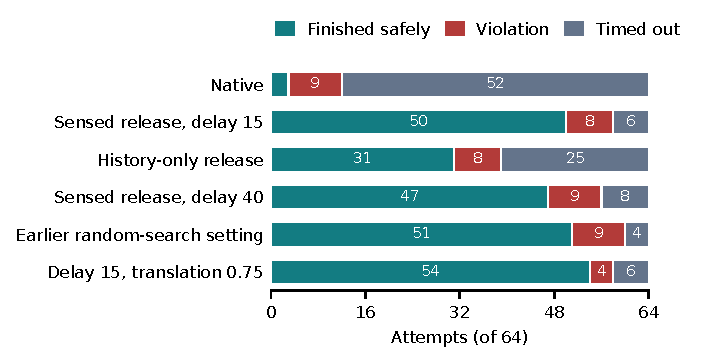
\includegraphics[width=\columnwidth]{unisafe-outcomes.pdf}
\caption{UNISafe confirmation, 64 attempts per setting on one host.
Removing grasp sensing (history-only release) turns completions into
timeouts. Counts below 4 are not printed.}
\label{fig:unisafe}
\Description{Stacked bars for six settings. Native finishes 3 of 64 and times
out 52 times. Sensed release finishes 50; history-only release finishes 31 with
25 timeouts; the best setting finishes 54.}
\end{figure}

\begin{table}[htbp]
\caption{UNISafe confirmation: 64 attempts per condition. $V$ is a physical
failure or boundary exit, $T$ a timeout, and $J$ completion time in seconds,
with 15 seconds assigned to failures and unfinished attempts.}
\label{tab:unisafe}\centering\small
\begin{tabular}{lrrrr}
\toprule
Setting & Safe completion & $V$ & $T$ & $J$ \\
\midrule
Native & 3/64 & 9 & 52 & 14.47 \\
Sensed release, delay 15 & 50/64 & 8 & 6 & 5.64 \\
Sensed release, delay 40 & 47/64 & 9 & 8 & 6.27 \\
Earlier random-search setting & 51/64 & 9 & 4 & 5.68 \\
Delay 15, translation 0.75 & 54/64 & 4 & 6 & 4.92 \\
History-only release & 31/64 & 8 & 25 & 10.57 \\
\bottomrule
\end{tabular}
\end{table}

The UNISafe study (Table~\ref{tab:unisafe}) has 590 attempts, including
four invalid renderer starts; all 384 confirmation attempts ran on one
physical host and are valid. The setting selected for speed is the same as the one selected for
completion, and no tested setting traded speed against completion, so the
study does not establish a useful speed/completion dial. High-completion settings still move the hand 70--83 cm
on average, so fewer filter interventions do not mean the agent stayed
still. Removing sensing increases capped completion time by 4.93 seconds,
with a corrected interval of $[2.86,6.89]$. Forty extra control steps after
success show that reaching the success condition and holding it are
different. Translation scaling holds success better, but that comparison
was post hoc.

The 16 October study ran on a different host and seed panel. Its selected
controllers finished safely in 54/64 (evolution), 56/64 (random search),
54/64 (policy gradient) and 55/64 (tuned fixed rule), against 2/64 for the
frozen policy; evolution's selection had seven physical failures and one
boundary exit, against six physical failures for the frozen policy. The
follow-up's delay-15 and delay-40 settings have the same parameters as that
study's evolution and fixed-rule selections, and its reference setting is
that study's random-search selection. The two studies are reported
separately and not pooled.

Appendix~\ref{app:jar} gives the ManiGuard Jar baseline, every numbered earlier Jar study and the details of the task 19 shield.

\subsection{Data and attempt counts}\label{app:data}
The experiment records, source hashes and private dataset revisions are
listed in the accompanying evidence manifest~\cite{mohan2026evidence}.
The task-16 and task-17 campaign folders of the TwoRoom and Reacher
datasets retain 10,180 attempts, including four failed engineering starts,
with raw traces, selected parameters, figures and replay videos; the same
datasets also hold the earlier task-12 and task-13 searches of
Appendix~\ref{app:evo-history}.
The PushT and Cube extension adds 2,028 attempts: two valid cohorts of 676,
one per task, each covering engineering, development, final, context and
timing attempts, and the superseded 676-attempt PushT cohort. Early engineering checks and
their work are recorded separately. Every scored stage has a verified source
archive. The earlier pre-data checks retain scripts, results and source-hash
records; their complete intermediate runtime sources were not recovered.
The \href{https://huggingface.co/datasets/Sachioster/SafetyDial-TwoRoom}{TwoRoom}
and \href{https://huggingface.co/datasets/Sachioster/SafetyDial-Reacher}{Reacher}
front pages provide a guided introduction before the technical records.
The \href{https://huggingface.co/datasets/Sachioster/SafetyDial-PushT}{PushT}
and \href{https://huggingface.co/datasets/Sachioster/SafetyDial-Cube}{Cube}
front pages link to the new matched comparisons and speed measurements.
The Jar tip-shield study preserves all 120 search attempts and 215 counted
confirmation attempts, plus one uncounted duplicate and one deliberate
repeat,
with recordings, monitor records, shield decisions and videos, in a private
ManiGuard dataset revision (Appendix~\ref{app:jar}).
The videos replay saved states or images; no new attempts were run to make
them. They illustrate behaviour, while the complete tables support the
performance claims. The datasets are currently private.
\section{Comparisons Across Margins and Recorded Examples}\label{app:visuals}
\subsection{Compare the planners at the same margin}
Figure~\ref{fig:dial-comparison} expands the familiar-layout result from Experiment One. Each point has 36 attempts: three layouts and twelve planner
seeds. It shows all four planners at all three tested margins in each task.
Feedback here is the Experiment One controller, not the learned mode selector from Experiment Two.

\begin{figure}[htbp]
\centering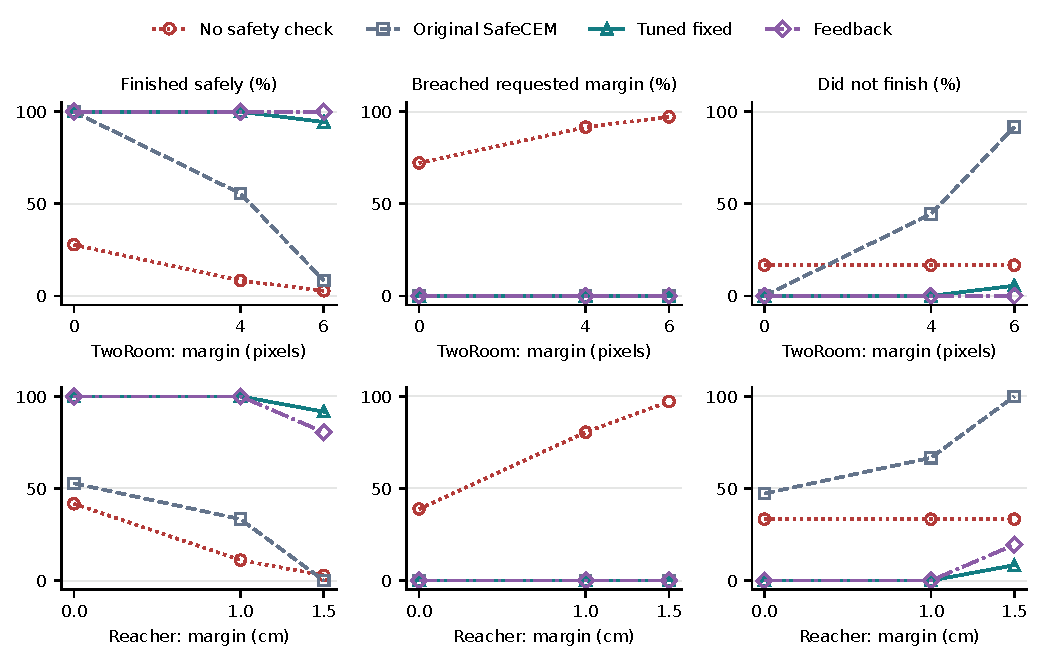
\includegraphics[width=.96\textwidth]{dial-comparison.pdf}
\caption{All four planners at every tested margin on the familiar layouts.
Higher safe completion is better; fewer breaches and unfinished attempts are
better. All 864 attempts move, and none ends in a controller failure. The
three checked planners have no observed breaches. Planning without the
safety check ignores the margin: it enters the danger region in 26/36
TwoRoom and 14/36 Reacher attempts at every margin, and its breaches grow
only because the same paths are judged against a wider margin. Its attempts were repeated and counted at each margin, but they are not independent evidence
across margins. Lines only join tested margins; several checked curves
overlap at zero breaches.}
\label{fig:dial-comparison}
\Description{Six panels compare No safety check, Original SafeCEM, Tuned
fixed and Feedback across three margins in TwoRoom and Reacher. Original
SafeCEM loses completion at larger margins, while tuned fixed and feedback
settings keep much more completion without observed breaches.}
\end{figure}

\textbf{How to read the figure.} To compare planners, read up and down at
one margin. To see what happens as the margin grows, follow one planner's
curve. The tuned fixed settings can differ between margins, but they do not
change during an attempt. Breaches and unfinished attempts can overlap,
because an attempt can breach the margin and still not finish, so one planner's
three percentages at one margin can add up to more than 100\%.

\textbf{What this adds.} Original SafeCEM becomes less useful as the margin
grows, while tuned fixed and feedback settings keep much more safe
completion. This is evidence on familiar layouts only. The new-case results
in Table~\ref{tab:fresh} compare only tuned fixed and feedback settings; they
do not include original SafeCEM or planning without the safety check.

\textbf{Fewer actions as well as more safe completions.} At the largest
margins (6 pixels in TwoRoom and 1.5 cm in Reacher), mean failure-capped
actions fall from 47.89 to 15.97 in TwoRoom and from 50.00 to 32.03 in
Reacher when tuned fixed settings replace original SafeCEM. Feedback scores
16.64 and 35.50. Every unfinished attempt counts as the full 50 actions,
and none of these checked groups has an observed breach. These are
averages over all attempts, not over successful attempts only, and they
count actions, not wall-clock time.

\subsection{Recorded examples and videos}
\begin{figure}[htbp]
\centering
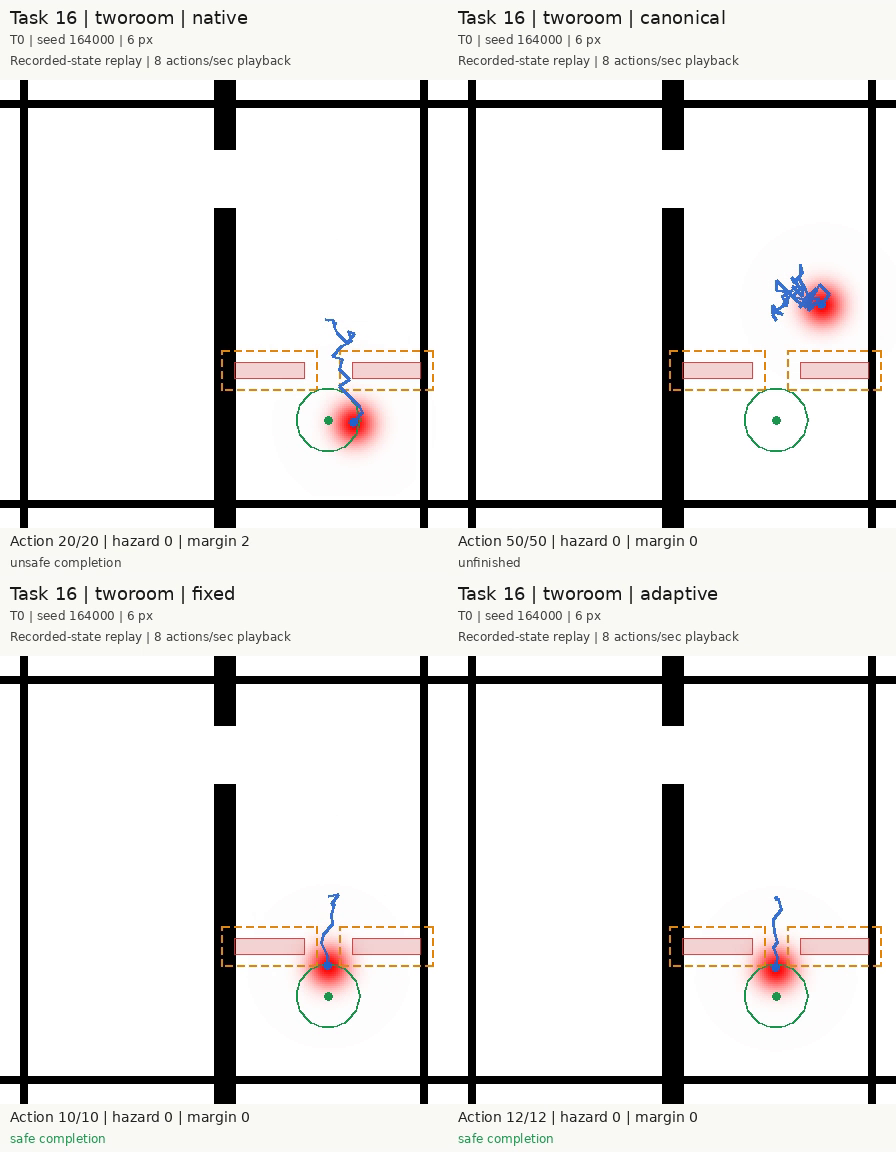
\includegraphics[width=.485\textwidth]{tworoom-four-methods.png}\hfill
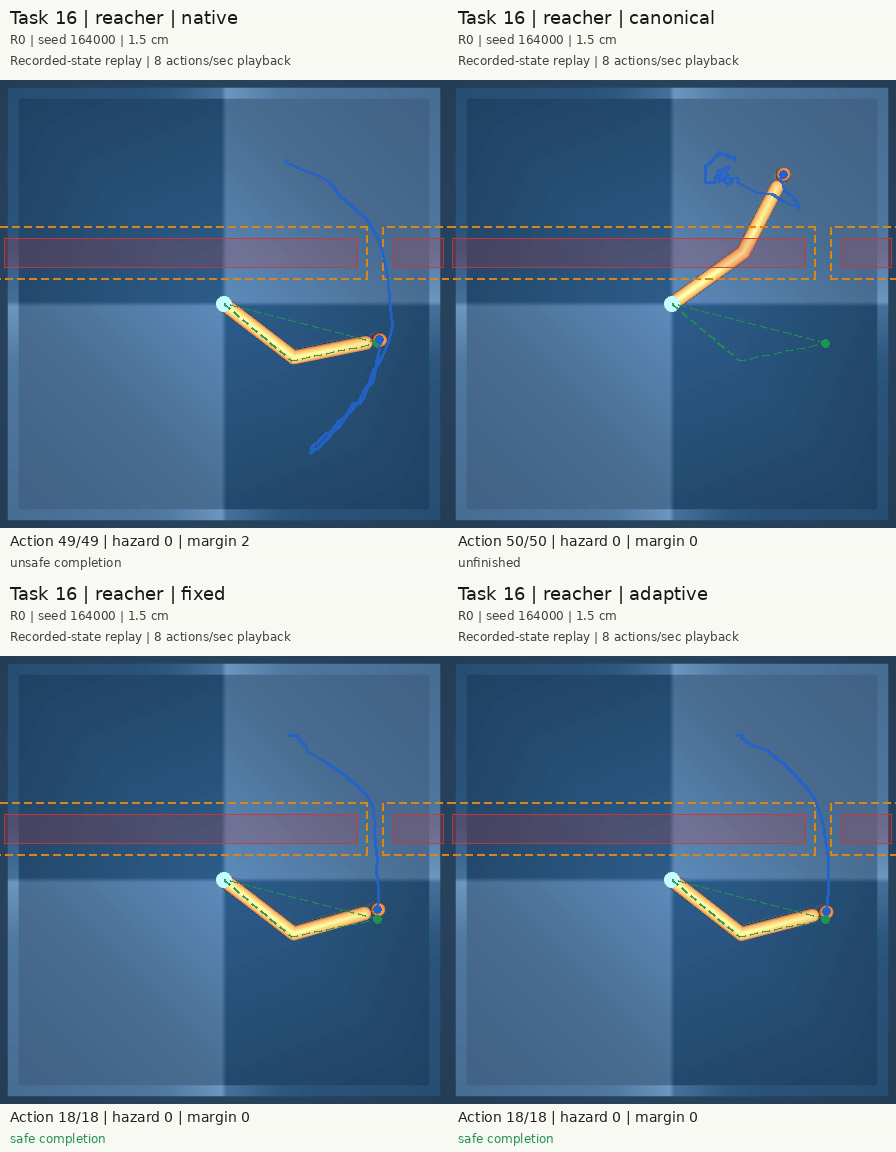
\includegraphics[width=.485\textwidth]{reacher-four-methods.png}
\caption{Recorded examples at the largest margin: TwoRoom on the left and
Reacher on the right, each from one matched case and planner seed. In each
image, upper left is No safety check, upper right Original SafeCEM, lower
left Tuned fixed and lower right Feedback. The burned-in panel labels use
code names: ``native'' is No safety check, ``canonical'' is Original
SafeCEM, ``fixed'' is Tuned fixed and ``adaptive'' is Feedback. In these
examples, planning without the safety check reaches the goal but breaches
the margin, Original SafeCEM does not finish, and Tuned fixed and Feedback
settings finish safely. Red outlined boxes mark the danger region, dashed
amber boxes the margin, blue the path and green the goal. These overlays are drawn for the reader and are not model inputs. The
burned-in footers give actions used, danger-region entries (hazard) and
margin breaches (margin); the red blob in TwoRoom is the agent. The images are saved dataset
pictures, not new attempts.}
\label{fig:paired-examples}
\Description{Two four-panel comparisons show the saved paths and final
states for No safety check, Original SafeCEM, Tuned fixed and Feedback.}
\end{figure}

\noindent Figure~\ref{fig:paired-examples} shows one matched case per task.
The links below and in Appendix~\ref{app:extension} open files in private
Hugging Face datasets; an account with access is required. The videos replay
recorded states at eight actions per second, so playback speed is not
planning speed. In both appendices, the examples illustrate behaviour; the
complete tables establish the results.

\begin{center}\small
\begin{tabularx}{\textwidth}{lXX}
\toprule
Comparison & TwoRoom & Reacher \\
\midrule
All four planners, familiar case &
\href{https://huggingface.co/datasets/Sachioster/SafetyDial-TwoRoom/blob/bed33b8967c30728dd76bfbdd4a046a6c34cedf8/campaigns/lewm16/videos/comparisons/A-paired-high-margin.mp4}{Play the four-planner video} &
\href{https://huggingface.co/datasets/Sachioster/SafetyDial-Reacher/blob/12624bc18843f0826566c4f1408d9028b2c61616/campaigns/lewm16/videos/comparisons/A-paired-high-margin.mp4}{Play the four-planner video} \\
Tuned fixed versus feedback, new case &
\href{https://huggingface.co/datasets/Sachioster/SafetyDial-TwoRoom/blob/bed33b8967c30728dd76bfbdd4a046a6c34cedf8/campaigns/lewm16/videos/comparisons/B-paired-high-margin.mp4}{Play the new-case video} &
\href{https://huggingface.co/datasets/Sachioster/SafetyDial-Reacher/blob/12624bc18843f0826566c4f1408d9028b2c61616/campaigns/lewm16/videos/comparisons/B-paired-high-margin.mp4}{Play the new-case video} \\
Selected optimizer controllers &
\href{https://huggingface.co/datasets/Sachioster/SafetyDial-TwoRoom/blob/bed33b8967c30728dd76bfbdd4a046a6c34cedf8/campaigns/lewm17/videos/comparisons/H-paired-high-margin.mp4}{Play the optimizer video} &
\href{https://huggingface.co/datasets/Sachioster/SafetyDial-Reacher/blob/12624bc18843f0826566c4f1408d9028b2c61616/campaigns/lewm17/videos/comparisons/H-paired-high-margin.mp4}{Play the optimizer video} \\
Guides, pictures and full results &
\href{https://huggingface.co/datasets/Sachioster/SafetyDial-TwoRoom}{Open the TwoRoom guide} &
\href{https://huggingface.co/datasets/Sachioster/SafetyDial-Reacher}{Open the Reacher guide} \\
\bottomrule
\end{tabularx}
\end{center}

In both optimizer comparison videos, all displayed controllers finish safely.
These clips do not show an advantage for evolution. As the main text
explains, a method may deploy a shared preset when that preset wins
validation.

The \href{https://huggingface.co/datasets/Sachioster/SafetyDial-PushT}{PushT}
and \href{https://huggingface.co/datasets/Sachioster/SafetyDial-Cube}{Cube}
datasets hold the task-18 comparison reported in Section~\ref{sec:extension}
and Appendix~\ref{app:extension}. They also hold older, separate studies:
the earlier SafeCEM probe on PushT (task 10) and the earlier Cube study
(task 14), which measured gripper reaching rather than cube moving. Appendix~\ref{app:evo-history} summarizes those older searches separately;
they are not pooled with any other result.

\section{PushT and Cube: Complete Matched Comparisons}\label{app:extension}
Table~\ref{tab:extension-all} gives every final comparison from
Section~\ref{sec:extension}. Each cell uses the same twelve cases and three
planner seeds. A breach and an unfinished task can occur in the same
attempt, so those columns can overlap.
\begin{table*}[t]
\caption{Task-18 final results, 36 attempts per cell: safe completions,
margin breaches, unfinished attempts, attempts that moved, and mean
failure-capped actions (lower is better; every unsafe or unfinished attempt
counts as 50 actions).}
\label{tab:extension-all}\centering\small
\begin{tabular}{llrrrrr}\toprule
Task and margin & Planner & Safe & Breaches & Unfinished & Moved & Capped actions \\
\midrule
PushT, 0 px & No safety check & 4 & 22 & 28 & 36 & 46.89 \\
 & Original SafeCEM & 4 & 0 & 32 & 36 & 48.14 \\
 & Tuned fixed & 19 & 0 & 17 & 36 & 35.22 \\
 & Feedback & 21 & 0 & 15 & 36 & 35.06 \\
\midrule
PushT, 6 px & No safety check & 3 & 23 & 28 & 36 & 47.44 \\
 & Original SafeCEM & 1 & 0 & 35 & 36 & 49.14 \\
 & Tuned fixed & 18 & 0 & 18 & 36 & 31.33 \\
 & Feedback & 17 & 0 & 19 & 36 & 31.81 \\
\midrule
PushT, 12 px & No safety check & 0 & 30 & 28 & 36 & 50.00 \\
 & Original SafeCEM & 2 & 0 & 34 & 36 & 49.53 \\
 & Tuned fixed & 19 & 0 & 17 & 36 & 35.42 \\
 & Feedback & 20 & 0 & 16 & 36 & 34.42 \\
\midrule
Cube, 0 cm & No safety check & 0 & 33 & 35 & 36 & 50.00 \\
 & Original SafeCEM & 0 & 0 & 36 & 36 & 50.00 \\
 & Tuned fixed & 13 & 0 & 23 & 34 & 37.08 \\
 & Feedback & 13 & 0 & 23 & 34 & 37.08 \\
\midrule
Cube, 0.5 cm & No safety check & 0 & 34 & 35 & 36 & 50.00 \\
 & Original SafeCEM & 1 & 0 & 35 & 36 & 49.72 \\
 & Tuned fixed & 13 & 0 & 23 & 35 & 36.47 \\
 & Feedback & 13 & 0 & 23 & 35 & 36.44 \\
\midrule
Cube, 1 cm & No safety check & 0 & 34 & 35 & 36 & 50.00 \\
 & Original SafeCEM & 0 & 0 & 36 & 36 & 50.00 \\
 & Tuned fixed & 12 & 0 & 24 & 35 & 37.86 \\
 & Feedback & 12 & 0 & 24 & 35 & 37.86 \\
\bottomrule
\end{tabular}
\end{table*}

\begin{table}[t]
\caption{Planning time at the largest margin, measured one attempt at a
time: two cases per planner, chosen in advance, with one new seed shared by
all four planners. Seconds per solve also count any failed final solve.
These timings describe two cases only and do not estimate a general speed
advantage.}
\label{tab:extension-time}\centering\small
\begin{tabular}{llrr}\toprule
Task & Planner & Seconds/solve & Safe / $n$ \\ \midrule
PushT & No safety check & 0.579 & 0/2 \\
PushT & Original SafeCEM & 0.597 & 0/2 \\
PushT & Tuned fixed & 0.410 & 0/2 \\
PushT & Feedback & 0.413 & 0/2 \\
Cube & No safety check & 0.637 & 0/2 \\
Cube & Original SafeCEM & 0.928 & 0/2 \\
Cube & Tuned fixed & 0.476 & 1/2 \\
Cube & Feedback & 0.531 & 1/2 \\
\bottomrule\end{tabular}
\end{table}

\paragraph{All work, including the superseded PushT cohort.}
Each task's valid cohort has 676 attempts: 8 engineering checks, 216
attempts to develop the fixed settings, 72 to develop feedback, 360 in the
final comparison (attempts without the safety check counted once, not once
per margin), 12 in the context panel that checks the protocol, and 8 timing
attempts. The two
valid cohorts together have 1,352 attempts. The superseded PushT cohort, run
before the reset repair, adds another 676, for 2,028 in all.
Table~\ref{tab:extension-work} also counts preliminary failed checks, model
warm-ups and reset work.
\begin{table}[t]\centering\small
\caption{Task-18 work across both valid cohorts, the superseded PushT cohort and preliminary checks.}
\label{tab:extension-work}
\begin{tabular}{lr}\toprule Quantity & Count \\ \midrule
Executed actions, excluding reset & 72,289 \\
Reset stabilization actions & 1,360 \\
Environment resets & 2,033 \\
All physics integrations & 1,840,851 \\
Of which simulator previews of candidates & 718,225 \\
Learned predictor steps & 660,428,575 \\
Model batch calls & 454,774 \\
\bottomrule\end{tabular}\end{table}
For the superseded PushT cohort and the preliminary checks, reset work is
reconstructed from the pinned reset code; the repaired cohort measures it
directly. Cube's 50 reset physics steps per attempt are already in its
physics count and are not added twice. Analytic path checks of candidates
are counted separately from true physics integrations; the dataset keeps
every counter.

Figure~\ref{fig:extension-dial} plots every final comparison in
Table~\ref{tab:extension-all} against the margin.
Figures~\ref{fig:extension-pusht} and~\ref{fig:extension-cube} show the
final observations from the first reserved case and first planner seed in
each task. The videos show the first two reserved cases with that seed,
chosen before any results were available, and compare all four planners at
the largest margin. The simulator images are saved observations; each video
panel also shows the goal image and a map of the safety boundary, with red
for the danger region and amber for the margin. The map is not an input to
LeWM. Cube targets can be above the table, so the Cube videos also report
the object's three-dimensional distance to its goal. The faint marker left
in the scene comes from data collection; it is not this case's target. A
case can be hard for every planner even when aggregate results improve
elsewhere.

The companion galleries show all twelve reserved cases with the same first
seed, failures included. A blue line traces the monitored pusher or
gripper, and a dashed line traces the object. Green marks the object goal,
with a separate green plus for PushT's pusher goal. Paths join saved action
states, while the safety score checks every physics step in between.
Playback is eight actions per second; Table~\ref{tab:extension-time} gives
the separate planning-time measurements.

\begin{figure*}[t]\centering
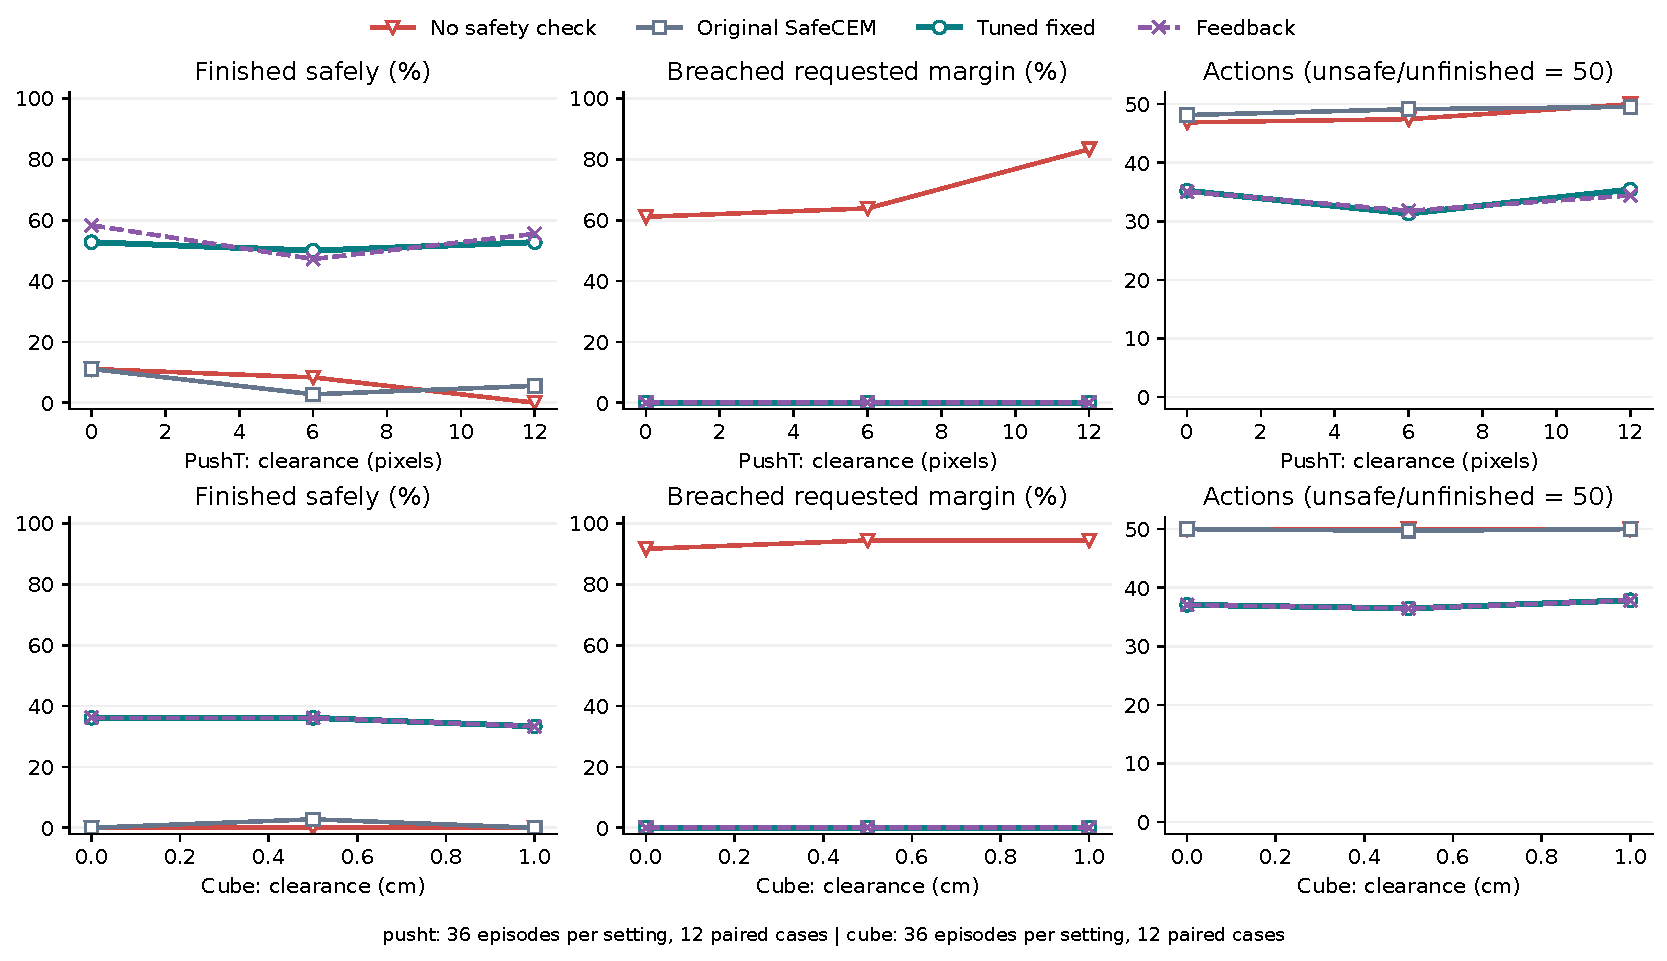
\includegraphics[width=.95\textwidth]{lewm18-comparison.pdf}
\caption{All task-18 final comparisons at matched margins. Each point has 36
attempts on twelve cases. Attempts without the safety check are recorded
once and scored at every margin. Failure-capped actions count every unsafe or unfinished attempt
as 50. Overlapping tuned fixed and feedback markers mean similar outcomes,
not missing data. The marker shapes differ from
Figure~\ref{fig:dial-comparison} in Appendix~\ref{app:visuals}, so use the
legend. In the axis labels, ``clearance'' means the margin; in the footer, ``episodes'' means attempts.}
\label{fig:extension-dial}
\Description{Safe completion, margin breaches and failure-capped actions for
the four planners in PushT and Cube at three margins.}
\end{figure*}
\begin{figure*}[t]\centering
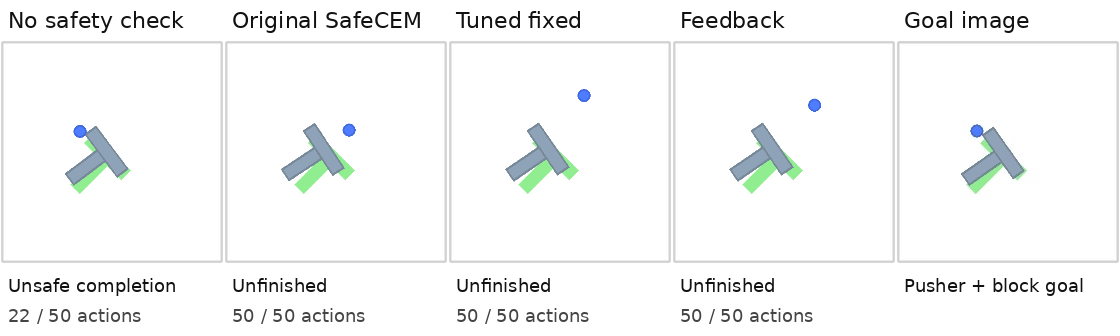
\includegraphics[width=\textwidth]{pusht-case-0-high-margin-paper.png}
\caption{PushT: final observations from the first reserved case and first
planner seed at the 12-pixel margin, beside the goal image. In this case no
checked planner finishes, and planning without the safety check finishes
in 22 actions but breaches the margin.}
\label{fig:extension-pusht}
\Description{Four PushT planners' final observations, outcomes and action counts beside their shared goal image.}
\end{figure*}
\paragraph{PushT videos and all-case galleries.}
\href{https://huggingface.co/datasets/Sachioster/SafetyDial-PushT/blob/ab3a1b4f7244227cf2b6cc972a38390b5cdfe6c4/campaigns/lewm18/media/pusht-case-0-high-margin.mp4}{Comparison video, case 1}.
\href{https://huggingface.co/datasets/Sachioster/SafetyDial-PushT/blob/ab3a1b4f7244227cf2b6cc972a38390b5cdfe6c4/campaigns/lewm18/media/pusht-case-1-high-margin.mp4}{Comparison video, case 2}.
\href{https://huggingface.co/datasets/Sachioster/SafetyDial-PushT/blob/ab3a1b4f7244227cf2b6cc972a38390b5cdfe6c4/campaigns/lewm18/media/pusht-trajectory-gallery-1.png}{All-case gallery, page 1}.
\href{https://huggingface.co/datasets/Sachioster/SafetyDial-PushT/blob/ab3a1b4f7244227cf2b6cc972a38390b5cdfe6c4/campaigns/lewm18/media/pusht-trajectory-gallery-2.png}{All-case gallery, page 2}.

\begin{figure*}[t]\centering
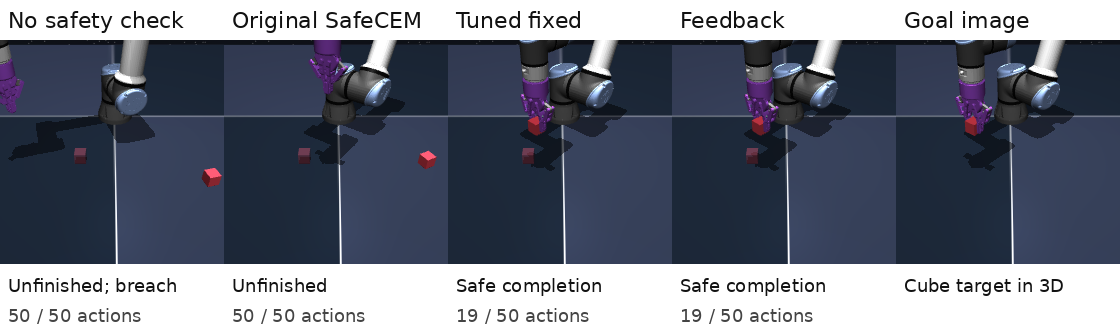
\includegraphics[width=\textwidth]{cube-case-0-high-margin-paper.png}
\caption{Cube: final observations from the first reserved case and first
planner seed at the 1 cm margin, beside the goal image. In this case tuned
fixed and feedback settings finish safely in 19 actions, original SafeCEM
does not finish, and planning without the safety check breaches the margin
without finishing.}
\label{fig:extension-cube}
\Description{Four Cube planners' final observations, outcomes and action counts beside their shared goal image.}
\end{figure*}
\paragraph{Cube videos and all-case galleries.}
\href{https://huggingface.co/datasets/Sachioster/SafetyDial-Cube/blob/49f10a4fc4fadcd520797a46d224a12d9bc299f7/campaigns/lewm18/media/cube-case-0-high-margin.mp4}{Comparison video, case 1}.
\href{https://huggingface.co/datasets/Sachioster/SafetyDial-Cube/blob/49f10a4fc4fadcd520797a46d224a12d9bc299f7/campaigns/lewm18/media/cube-case-1-high-margin.mp4}{Comparison video, case 2}.
\href{https://huggingface.co/datasets/Sachioster/SafetyDial-Cube/blob/49f10a4fc4fadcd520797a46d224a12d9bc299f7/campaigns/lewm18/media/cube-trajectory-gallery-1.png}{All-case gallery, page 1}.
\href{https://huggingface.co/datasets/Sachioster/SafetyDial-Cube/blob/49f10a4fc4fadcd520797a46d224a12d9bc299f7/campaigns/lewm18/media/cube-trajectory-gallery-2.png}{All-case gallery, page 2}.

% Task-18 full methods, moved from the main text. Summary in lewm18-methods.tex.
\section{PushT and Cube Methods}\label{app:extension-methods}
\subsection{Tasks, cases and methods}
In Cube, success means the cube's centre comes within 4 cm of the target.
(An earlier Cube probe in our records tested only gripper reaching, so it is
not evidence for this goal.) Each task uses its own frozen LeWM checkpoint.
Each case takes a start image and a goal image 25 recorded actions apart in
the task's pinned demonstration dataset, places a forbidden band across the
straight line from start to goal with an off-centre gap, and keeps the start
and goal outside the enlarged danger region. Development and
final cases come from different demonstrations. A 0 margin keeps only the
original danger region. Native planning ignores the margin, so its attempts
are recorded once and scored at all three margins; these are three views of
the same attempts, not three independent samples.

The allowance is 50 executed actions, with a replan after every five.
Original SafeCEM uses 30 CEM iterations, 300 candidates and five blocks of
look-ahead. Shorter look-ahead receives more candidates under the same
allowance of 1,500 predictor steps per iteration. We report actual model
work separately, because early completion, failed replans and the extra
prediction for the chosen plan change the work used.

\subsection{Selection}
The Feedback controller uses latent progress and prediction error to change look-ahead, sampling
spread and candidate reuse; it cannot weaken the margin. For each margin, six
fixed configurations are compared on six development cases with two seeds.
Four Feedback presets then use the same six cases and one seed. Selection
first maximizes safe completion, then breaks ties by fewer failure-capped
actions, less model work and finally list order. Feedback builds on the
fixed-setting selection and uses another 72 development attempts per task,
so its tuning cost is higher, not equal.

\subsection{What the checks and speed measurements mean}
The safety rule covers only the pusher centre in PushT and the gripper pinch
point in Cube. It does not certify the moved object, the arm or the whole
robot against collision. In PushT, the checker uses the known pusher
dynamics and tests every physics step. In Cube, it ranks candidates with an
approximate path, then tests the first five actions of up to eight
candidates in the true simulator. Every such preview counts toward the work
totals, and the full simulator state is restored before the next preview or
the real action. If no preview passes, the attempt ends as a controller
failure; there is no unchecked fallback.

PushT keeps the pinned environment's own success test, which requires the
pusher position, block position and block angle to be close to the goal; we
do not report shape overlap. Cube's goals come from LeWM's dataset pairs, not
the full official five-goal OGBench evaluation. As a small protocol check,
native planning also ran on twelve separate pairs per task executing all
25 planned actions before replanning, as the reference planner does, without
a danger region or checker. It completes 11/12 PushT pairs and 10/12 Cube
pairs, but seven of the Cube pairs already meet the object goal at reset, so
this panel must not replace the reserved cases.

Speed is scored in failure-capped actions (Section~\ref{sec:success}): a safe
completion costs the actions it used, and every unsafe or unfinished attempt
costs 50, so early failure cannot look fast. Mean actions among successful
attempts are secondary and are reported with their own counts. A separate
run, one attempt at a time, measures actual planning time on the first two
final cases at the largest margin, with a new shared seed. Video playback
speed says nothing about computation time. Uncertainty intervals resample
whole cases, keeping each case's seeds and paired planners together.

\subsection{The PushT reset repair}
A review before publication found that resetting PushT moves the simulator
slightly, but the checker in our first cohort started from the state before
the reset. We made the checker start from the state that reset returns and
repeated the full protocol, including development selection, with the same
cases and candidate configurations. The first cohort's 676 attempts are kept
and counted in the work totals, but excluded from the performance results.

% Task-19 appendix: ManiGuard Jar history, protocol, search, confirmation details and integrity.
% Numbers come from progress/receipts/19-evo-adapter-results.md, configs/evo19/protocol.json,
% outputs/evo19/search/state.json and outputs/evo19/analysis/{summary,mechanism,revalidation}.json.
\section{ManiGuard Jar Details}\label{app:jar}
\subsection{Earlier Jar studies}\label{app:jar-history}
Task 19 is the latest of several attempts to help the same frozen policy on
Jar. The policy is ManiGuard's released Jar fine-tune of
$\pi_{0.5}$~\cite{black2025pi05,peng2026maniguard}, running in the
OmniGibson simulator of BEHAVIOR-1K~\cite{li2023behavior1k}. The baseline
replication (task 1) ran all 26 Jar scenes (ManiGuard numbers them as tasks;
we say scenes to keep ``task'' for our study numbers) with 20 Hz control, eight executed
targets per 16-target chunk, $256\times256$ cameras, a 2,000-step horizon and a
ten-step goal hold. It recorded 24 safe successes, seven unsafe successes, 37
safe failures and 36 unsafe failures in 104 attempts, with 43 counted violations and 103 engaged attempts. The
benchmark counts a violation only after first contact; a raw violation, used
from task 5 on, is any rule broken at any step. Of the 24 safe successes, 23 also closed
the jar before lifting it. Of the 43 violations, 33 were tips, eight lifted
the jar before closure and two did both at once.

Figure~\ref{fig:jar-history} places each later intervention beside the native
arm of its own study. The studies use different seeds, scenes and hosts, so
they are never pooled. A retreat triggered when the arm stopped moving (task 3) changed
neither safe success nor violations. An execution adapter with joint feedback
(task 5) and latent steering in the style of DSRL (task 7) did not help.
Slower joint targets passed a 12-attempt screen, 6/12 against 4/12, but not
their fresh-seed confirmation, 2/12 against 2/12 (task 8). The task 15 screen
favoured speed projection, 9/16 against 5/16 strict safe completions, but a
one-sided Fisher test gives $p=0.14$, and choosing among thirty-two sampled chunks reached only 3/16 or 4/16. Its confirmation lost two rented hosts and was never
completed; a partial mirror of it could not be verified and is not used here.
Task 15 also replayed stored observations: of 254 executed chunks recorded in
task 7 that failed a 0.10 m/s check (85 of them from the native arm), 122 had
a passing alternative among sixteen fresh policy samples. The speed-limit
stages of task 19 did not reproduce the screen's gain
(Section~\ref{sec:jar}). Task 3 counts benchmark safe success, which does
not require closing the jar first; the other rows use strict safe completion.

\begin{figure*}[t]
\centering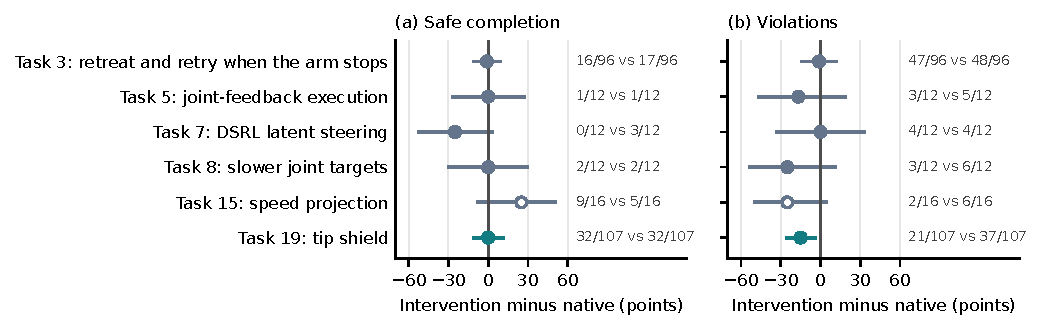
\includegraphics[width=\textwidth]{jar-history.pdf}
\caption{Every completed numbered Jar intervention study since the task 1
replication, plus the task 15 development screen, each against the native
policy in the same study, never pooled; earlier archived pilots are not shown. Dots are differences in percentage
points; lines are 95\% Newcombe intervals for two independent proportions,
which ignore pairing. The hollow marker is a development screen. Counts are
intervention versus native. Task 3 uses benchmark safe success and counted
violations; the others use strict safe completion and raw violations. Only
the task 19 violation interval excludes zero.}
\label{fig:jar-history}
\Description{A dot-and-interval chart with six studies. Safe completion
differences all have intervals spanning zero. For violations, only the task 19
tip shield has an interval entirely below zero.}
\end{figure*}

\subsection{Task 19 protocol}
The policy is the $\pi_{0.5}$ Jar checkpoint 7400, unchanged, served with
ManiGuard's evaluator at commit 6bf4c61 and its Jar configuration: 20 Hz joint
control, eight executed targets per 16-target chunk, $256\times256$ cameras, a
2,000-control horizon and a ten-step goal hold. The protocol was frozen at
22:10 UTC on 26 October 2026, before any search attempt. Its primary endpoint
is strict safe completion, evolved adapter minus native (the shield after
amendment 3), by a one-sided Fisher exact
test with Wilson intervals. Raw violation attempts were listed as a secondary
endpoint. Search attempts are training data, not effect estimates, and no
result is pooled with earlier Jar studies.

The search ran four stages, each with pycma~\cite{hansen2019pycma} in unit
coordinates, starting at the centre of the box with step size 0.25 (0.2 in
stage 2). Stage 1 evolved a near-jar speed projection with three genes: a speed
limit (0.03 to 0.30 m/s, log scale), a near radius (0.10 to 0.35 m) and a weight
for steps that move away from the jar (0 to 1). It tested eight candidates per
generation and scored four points for a strict safe completion, two for no
violation and one for grasping the jar. Stage 2 fixed the weight at one and
dropped the violation term. Stages 3 and 4 evolved the tip shield: tilt limit
$3+12u_0$ degrees and retreat distance $0.02+0.10u_1$ m, scored as four points
for a strict safe completion plus one point for no violation. Stages 2 to 4
tested six candidates per generation. Stage 3 counted contact only at the query control; stage 4
counted it over the eight controls up to the query, because the contact count
flickers during a push. Candidate $i$ of stage 4 generation $g$ ran scene $(0,3,6,9)_{i \bmod 4}$ with seed $195000+10g+i$. After eight generations the
distribution mean was frozen as the shield.

\begin{table*}[t]
\caption{Task 19 protocol amendments, all times UTC on 26 and 27 October 2026.
The last column states which confirmation outcomes existed when each change was
recorded, by host finish time; the dated records list 17 native outcomes as
visible at amendment 2 and 60 shielded at amendment 7. No amendment re-scored a finished attempt or changed the primary endpoint;
amendments 2 to 4 changed the search, its score and with it the adapter the
evolved arm would deploy (the shield from amendment 3), and amendments 3 and
4 redefined the optional hand-set arm that amendment 6 cancelled.}
\label{tab:jar-amendments}\centering\small
\begin{tabularx}{\textwidth}{rlXl}
\toprule
& Time & Change & Confirmation attempts finished \\
\midrule
1 & 22:37 & Confirmation panel enlarged from 48 to 72 pairs (seeds 193000--193017), interleaved in seed order; the optional hand-set speed-limit arm scheduled after both primary arms & 0 native, 0 shield \\
2 & 23:35 & Stage 1 closed as exploratory; stage 2 fixes the retreat weight at one & 18 native, 0 shield \\
3 & 23:51 & Stage 2 closed as exploratory; stage 3 evolves the tip shield & 21 native, 0 shield \\
4 & 23:59 & Stage 3 closed as a pilot; stage 4 counts contact over eight controls & 22 native, 0 shield \\
5 & 00:00 & Exact tests fixed for the listed violation endpoint (Fisher, Barnard, exact McNemar) & 22 native, 0 shield \\
6 & 01:07 & Hand-set arm cancelled; panel extended by seeds 193018--193029 to 120 pairs & 47 native, 0 shield \\
7 & 01:48 & Scheduling only: remaining jobs run in pair order so a time cut leaves complete pairs & 48 native, 62 shield \\
\bottomrule
\end{tabularx}
\end{table*}

\begin{figure*}[t]
\centering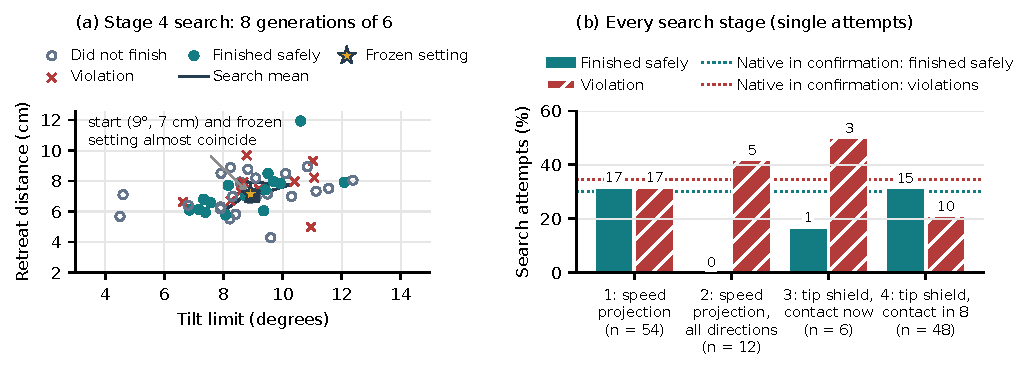
\includegraphics[width=\textwidth]{evo19-search.pdf}
\caption{The task 19 search. (a) Every stage 4 candidate, coloured by its single
attempt's outcome, with the path of the CMA-ES mean. The mean ended close to its
hand-chosen start. (b) Outcomes of each search stage. The dotted lines mark the
native policy's rates in confirmation, which used different seeds; search
attempts are training data, not effect estimates.}
\label{fig:jar-search}
\Description{Left: a scatter of 48 candidate settings around 9 degrees and 7 cm
with the search mean wandering near its start. Right: bars of safe completion and
violation rates for the four search stages.}
\end{figure*}

\subsection{Confirmation details}\label{app:jar-confirm}
Table~\ref{tab:jar-detail} breaks the confirmation down by scene and by
outcome. Scene 9 is the hardest for both arms. The rule-replay columns
apply the frozen trigger to each recording: at a policy query before any
violation, tilt at least 8.92 degrees and robot contact in the last eight
controls. For the shield arm the replay fires in exactly the 50 attempts that logged a
retreat (255 retreat chunks in all, each also reproduced by the per-decision
replay in the integrity checks). For the native arm it marks where the shield
would first have acted; after that point the two arms would diverge, so it
is not a prediction of the shielded outcome. Violations happen before the jar
is closed in 11 native and 7 shielded attempts, and after closure in 26 and 14.

\paragraph{Intervals and endpoints.} Differences are shield minus native with
95\% Newcombe hybrid-score intervals~\cite{newcombe1998interval}, built
from Wilson score intervals~\cite{wilson1927probable}, which
match the unpaired Fisher and Barnard tests. Strict safe completion, the
primary endpoint, differs by 0.0 points, $[-12.1,12.1]$; violations differ by
$-15.0$ points, $[-26.3,-3.0]$. The protocol listed six secondary endpoints and fixed no multiplicity
correction; amendment 5 named raw violations the key secondary. Bonferroni
over the primary and that endpoint asks for $p<0.025$, which the violation
test meets (Fisher $p=0.010$, Barnard $p=0.008$); over all seven listed
endpoints it asks for $p<0.0071$, which it does not. The primary endpoint
shows no effect. The original 72-pair panel alone shows the same pattern, 25
against 13 violations and 22 against 25 strict safe completions. One shielded
attempt (scene 9, seed 193026) has no native partner because its native
attempt did not finish before the stop; it was a violation, and adding it gives 22/108.

\paragraph{Post hoc checks on timing.} The shield was designed at amendment 3
(23:51 UTC) and frozen at 01:07:13 UTC, 42 seconds before amendment 6 was
recorded, while native confirmation
attempts were already finishing (Table~\ref{tab:jar-amendments}). The violation test was fixed before any shielded attempt, but the design did
use native outcomes: amendment 3 records that five native confirmation violations were inspected
together with 17 search violations; by then 21 native attempts, seven of them
violations, had finished. Dropping the 21 pairs whose native
attempt finished before amendment 3 leaves 30/86 against 15/86 violations,
$-17.4$ points, $[-29.9,-4.3]$, one-sided Fisher $p=0.007$, with 22 against 23
strict safe completions. Dropping the 45 pairs whose native attempt finished
before the freeze leaves 20/62 against 12/62, $-12.9$ points, $[-27.6,2.5]$,
$p=0.075$, with 17 against 14 strict safe completions. Both keep the
direction; the second is not significant alone. These cuts are post hoc and
descriptive.

\paragraph{Outcome changes within pairs.} Table~\ref{tab:jar-transitions}
crosses each pair's native outcome with its shielded one. Because attempts
are not deterministic per seed, a cell is not a causal effect on that
scene. In 22 pairs the native attempt broke a rule and the shielded one did not, and
in six the reverse; 12 pairs combine a native safe completion with a shielded
stall, and 8 combine a native violation with a shielded safe completion.

\begin{table}[t]
\caption{Outcomes within the 107 matched pairs: rows native, columns shield.}
\label{tab:jar-transitions}\centering\small
\begin{tabular}{lrrrrr}
\toprule
Native $\downarrow$ / shield $\rightarrow$ & Safe & Viol. & Stall & Never & Total \\
\midrule
Strict safe & 15 & 3 & 12 & 2 & 32 \\
Violation & 8 & 15 & 11 & 3 & 37 \\
Stalled after closing & 6 & 0 & 14 & 6 & 26 \\
Never closed & 3 & 3 & 3 & 3 & 12 \\
\midrule
Total & 32 & 21 & 40 & 14 & 107 \\
\bottomrule
\end{tabular}
\end{table}

\begin{table}[t]
\caption{Jar confirmation by scene and by outcome; each N / S cell gives native /
shield. ``Rule
fires'' counts attempts in which the frozen trigger holds at a query before any
violation.}
\label{tab:jar-detail}\centering\small
\begin{tabular}{lrrr}
\toprule
By scene & Pairs & Strict safe (N / S) & Violations (N / S) \\
\midrule
Scene 0 & 27 & 14 / 9 & 9 / 7 \\
Scene 3 & 27 & 7 / 11 & 8 / 2 \\
Scene 6 & 27 & 10 / 10 & 7 / 4 \\
Scene 9 & 26 & 1 / 2 & 13 / 8 \\
\midrule
By outcome & & Attempts (N / S) & Rule fires (N / S) \\
\midrule
Strict safe & & 32 / 32 & 9 / 10 \\
Violation & & 37 / 21 & 34 / 17 \\
Stalled after closing & & 26 / 40 & 10 / 19 \\
Never closed & & 12 / 14 & 4 / 4 \\
\bottomrule
\end{tabular}
\end{table}

\subsection{Integrity, cost and preservation}
Each confirmation attempt was validated on its host from the recording and
the monitor's record, including an exact replay of every shield decision.
All 215 counted confirmation attempts were validated again on the workstation
and match both the stored records and the host checks. One worker ran a
shield job a second time straight after its counted attempt had finished. The
duplicate is excluded; it ended without finishing, so counting it instead
would lower the shield's strict safe count by one and change no violation
count. A deliberate repeat of one native attempt closed the jar and tipped
late, where the original tipped before closure, which shows that attempts are
not deterministic per seed. The run used eight single-GPU rentals (seven RTX
3090 and one RTX 4090, several replaced early when slow or failing) between
21:43 and 02:57 UTC, at a conservative estimated cost of US\$8.58. Every attempt
is preserved in the private dataset
\texttt{Sachioster/maniguard-jar-replication-20261022} under
\texttt{evo19/}, revision \texttt{98e8fe31}, with 5,564 files re-downloaded
and checked by SHA-256.

% Exploratory NSGA-II versus random search, tasks 10, 12, 13 and 14 (stage C searches).
% Numbers come from progress/receipts/{10-safecem-C2-search.md,12-tworoom-C-search.md,
% 13-reacher-C-search.md,14-cube-C-search.md} and their freezes, cross-checked against
% outputs/safecem10/analysis/stageC2-summary.json and outputs/{tworoom12,reacher13,cube14}/
% analysis/stageC-summary.json ("methods" and "pairwise"; wins count strict NSGA-II > random
% over the 3 x 3 run pairs). Task 10 numbers are from stage C2, the rerun after stage C was
% paused at generation 0. Written for the one-column appendix layout.
\section{Earlier Exploratory Evolutionary Searches}\label{app:evo-history}
Before the main optimizer comparison (task 17, Table~\ref{tab:primary}), four
exploratory studies compared NSGA-II~\cite{deb2002nsga2}, a multi-objective evolutionary
algorithm, with random search. Both methods tuned the settings of SafeCEM. SafeCEM is a planner with a
safety check, not an evolutionary method; evolution was only this outer search over
its settings. The tasks were PushT with a gapped wall across the pusher's route
(task 10), TwoRoom (task 12), Reacher (task 13) and Cube (task 14). Task 14 used an
earlier gripper-reaching goal, not the object-moving goal of
Section~\ref{sec:extension}.
% source: progress/receipts/10-safecem-C2-freeze.json:139 (wall with a gap), :93 (success =
% block coverage); progress/receipts/14-cube-A-engineering.md:21-22 (reach task: pinch point
% within 0.04 m of the goal); experiments/helpers/{tworoom12,reacher13,cube14}_planner.py:1
% ("SafeCEM on ...").
Each search tuned five settings, with ranges scaled to each task: the margin at the
first predicted block and its change per later block, the look-ahead horizon (3 to 7
blocks), the elite fraction, and a tolerance on the summed predicted penetration of the
danger region plus margin. Unlike the main experiments, the margin itself was searched.
Two objectives were minimized: exposure, the fraction of saved states inside the danger
region, and steps to success, counted as 50 when the attempt failed. Each front was
scored by its hypervolume up to the reference point (1, 50). This score rewards low
exposure rather than requiring zero entries into the danger region, and the tolerance let the check accept
small predicted penetrations. Each method ran three independent searches per task. One
search evaluated 96 settings (12 per generation for 8 generations) on three seeds each,
288 attempts. Its final front, at most six settings, was then rerun on ten new seeds of
the search layout and ten seeds of a held-out layout.
% source: progress/receipts/10-safecem-C2-freeze.json:278-312 (objectives exposure and J,
% reference point [1.0, 50.0], genes d0, d1, horizon 3..7, topk_frac, tol), :230-234,253,265-277
% (population 12, 8 generations, 3 replicates, 3 seeds per candidate, final seeds 400..409,
% front cap 6); progress/receipts/12-tworoom-C-search.md:14-19,72-73 ("96 candidates of 3 seeds
% per run"); 13-reacher-C-search.md:14-19; 14-cube-C-search.md:14-20; same objectives and
% reference point in 12-tworoom-C-v1.json:274-281, 13-reacher-C-v1.json:248-255,
% 14-cube-C-v1.json:245-252. Exposure = share of saved states inside the true boxes
% (experiments/helpers/safecem10_geometry.py:111); tolerance = summed penetration of the inflated
% boxes still accepted as feasible (safecem10_planner.py:89-90,175-179); hypervolume = exact
% dominated area (safecem10_evo.py:194-195). Totals 3032, 2892, 2792, 2872 attempts (receipts
% lines 4-5) equal 9 x 288 search attempts plus 20 per final setting.

\begin{table}[htbp]
\caption{Exploratory NSGA-II versus random search. Hypervolume (HV, higher is better, at
most 50) of each final front, mean $\pm$ standard deviation over three runs per method,
on new seeds of the search layout (fresh) and on a held-out layout; standard deviations
are population values with $n=3$. Wins give, out of the nine pairings of one NSGA-II run
with one random-search run, how many NSGA-II won on HV. HV scales differ
by task, so compare only within a row. A third method, a fixed grid, is omitted.}
\label{tab:evo-history}\centering\small
\begin{tabular}{@{}lrrrrcc@{}}
\toprule
 & \multicolumn{2}{c}{Fresh HV} & \multicolumn{2}{c}{Held-out HV} & \multicolumn{2}{c}{NSGA-II wins} \\
\cmidrule(lr){2-3}\cmidrule(lr){4-5}\cmidrule(l){6-7}
Task & NSGA-II & Random & NSGA-II & Random & Fresh & Held out \\
\midrule
% source: progress/receipts/10-safecem-C2-search.md:32 (NSGA-II 6.23 +/- 2.89, 8.64 +/- 2.27),
% :33 (random 9.18 +/- 3.47, 5.32 +/- 3.86), :42 (wins 3/9 fresh, 7/9 held out)
PushT (10) & $6.2\pm2.9$ & $9.2\pm3.5$ & $8.6\pm2.3$ & $5.3\pm3.9$ & 3/9 & 7/9 \\
% source: progress/receipts/12-tworoom-C-search.md:25 (NSGA-II 32.83 +/- 1.80, 35.57 +/- 0.87),
% :26 (random 37.00 +/- 0.22, 38.10 +/- 0.22), :29-30 (random beat NSGA-II in 9 of 9 on both)
TwoRoom (12) & $32.8\pm1.8$ & $37.0\pm0.2$ & $35.6\pm0.9$ & $38.1\pm0.2$ & 0/9 & 0/9 \\
% source: progress/receipts/13-reacher-C-search.md:25 (NSGA-II 17.20 +/- 6.49, 11.67 +/- 0.68),
% :26 (random 16.20 +/- 5.55, 14.13 +/- 4.43), :32-33 (NSGA-II 5 of 9 on both)
Reacher (13) & $17.2\pm6.5$ & $16.2\pm5.6$ & $11.7\pm0.7$ & $14.1\pm4.4$ & 5/9 & 5/9 \\
% source: progress/receipts/14-cube-C-search.md:26 (NSGA-II 1.20 +/- 0.62, 1.13 +/- 0.90),
% :27 (random 4.42 +/- 3.59, 12.23 +/- 6.39), :33-34 (NSGA-II 1 of 9 fresh, 0 of 9 held out)
Cube reaching (14) & $1.2\pm0.6$ & $4.4\pm3.6$ & $1.1\pm0.9$ & $12.2\pm6.4$ & 1/9 & 0/9 \\
\bottomrule
\end{tabular}
\end{table}

NSGA-II did not consistently beat random search (Table~\ref{tab:evo-history}). Random
search won every TwoRoom comparison and all but one on Cube, and Reacher was a tie. On
PushT, NSGA-II trailed on new seeds but led on the held-out layout; with three runs per
method and standard deviations of 2 to 4, neither difference is conclusive. The study
records suggest the TwoRoom and Cube losses were partly due to selecting on only three
noisy seeds per setting.
% source: progress/receipts/10-safecem-C2-search.md:66-69 (fresh favours random, held out
% favours NSGA-II, sd 2 to 4, neither conclusive); 13-reacher-C-search.md:58-60 (tie);
% 12-tworoom-C-search.md:65-66,72-75 ("selection on 3 noisy seeds also cost it");
% 14-cube-C-search.md:64-68,81-83 ("its selection was misled by noise").
These studies were exploratory. Their objectives, budgets and optimizer differ from
task 17, so we neither pool them nor compare them across tasks. They show only that
NSGA-II gave no reliable gain over random search at these small budgets, not that
evolution cannot help.

\end{document}
